% =============================================================================
% APPENDIX AAA: THEORY OF AGGREGATION LEVELS
% =============================================================================
% Module: BCM2_00_META (Foundational Theory)
% Version: 1.1 (January 2026)
%
% The most fundamental appendix: Defines the level structure on which
% all EBF utility calculations operate.
%
% =============================================================================
% CROSS-REFERENCE STRUCTURE
% =============================================================================
%
% Appendix AAA provides the theoretical foundation for:
% - Appendix C (FEPSDE Matrix): Utility at each level
% - Chapter 9 (Context): Ψ modulates level salience
% - Chapter 10 (Welfare): Aggregation across levels
% - Chapter 11 (Awareness): Level-specific awareness
%
% =============================================================================

\chapter{Theory of Aggregation Levels}
\label{app:aggregation-levels}

\begin{abstract}
This appendix develops the fundamental theory of aggregation levels in EBF.
Rather than assuming arbitrary levels (individual, household, nation...), we derive
the level structure from first principles: \textbf{What can have utility?} and
\textbf{What defines a level?} The answer leads to a recursive, self-similar
structure where KNU and IDN \emph{define} levels rather than merely operating
within them. The theory extends from the individual (Level 0) to all sentient
beings across all time (Level $\infty$).
\end{abstract}

%==============================================================================
% HEADER BLOCK (Required)
%==============================================================================

\begin{tcolorbox}[colback=red!5!white, colframe=red!75!black, 
    title=\textbf{CORE Appendix: Aggregation Levels}]

\begin{tabular}{@{}ll@{}}
\textbf{Appendix:} & AAA (Aggregation Levels) \\
\textbf{Category:} & CORE \\
\textbf{CORE Question:} & \textbf{WHO} --- Who can have utility? \\
\textbf{Scope:} & A1 (Foundational Theory) \\
\textbf{Version:} & 1.1 \\
\textbf{Last Updated:} & January 2026 \\
\textbf{Dependencies:} & None (foundational) \\
\textbf{Dependents:} & Appendix C (dimensions at each level) \\
 & Appendix B (complementarity across levels) \\
 & Appendix V (context by level) \\
 & Appendix AU (awareness at each level) \\
 & Appendix AV (willingness at each level) \\
\textbf{Output:} & Level hierarchy $L \in \{0, 1, 2, 3, 4, 5, \infty\}$ \\
\end{tabular}

\vspace{0.3cm}

\textbf{The 9C CORE Framework:}
\begin{center}
\small
\begin{tabular}{@{}cllc@{}}
\toprule
\textbf{C} & \textbf{Question} & \textbf{Appendix} & \textbf{Output} \\
\midrule
\textbf{WHO} & \textbf{Who has utility?} & \textbf{AAA (this)} & $L \in \{0...\infty\}$ \\
WHAT & What is utility? & C & FEPSDE $d$ \\
HOW & How do they interact? & B & $\Gamma, \Lambda, \delta$ \\
WHEN & When does context matter? & V & $\boldsymbol{\Psi}$ \\
WHERE & Where do numbers come from? & BBB & $\Theta, E(\theta)$ \\
\midrule
AWARE & How salient is utility? & AU & $A(\cdot), U_{eff}$ \\
READY & How willing to act? & AV & $WAX, \theta$ \\
STAGE & Where in the journey? & AW & $\varphi \in \{1,...,5\}$ \\
\bottomrule
\end{tabular}
\end{center}

\end{tcolorbox}

%==============================================================================
% FORMAL COMPLIANCE BLOCK
%==============================================================================

% --- Terminology Reference ---
\begin{tcolorbox}[colback=gray!5!white, colframe=gray!50!black]
\textbf{Terminology:} See Appendix G (Glossary) for standard definitions.
Key terms in this appendix: Aggregation level ($L$), welfare hierarchy,
INU (Individual Utility), KNU (Collective Utility), IDN (Identity Utility),
level salience $\alpha^L(\Psi)$, membership function $M^L$.
\end{tcolorbox}

% --- Chapter Linkage Box ---
\begin{tcolorbox}[colback=green!5!white, colframe=green!75!black,
    title=\textbf{Chapter References}]

\textbf{Primary Chapter:} Ch. 10.8 (Aggregate Welfare Function)
\begin{itemize}[nosep]
    \item Hierarchical aggregation from Level 0 to Level $\infty$
    \item Cross-level complementarity $\gamma^{cross}_{L,L'}$
\end{itemize}

\textbf{Secondary Chapters:}
\begin{itemize}[nosep]
    \item Ch. 9 (Context): Level salience function $\alpha^L(\Psi)$
    \item Ch. 10.1 (Three Categories): INU/KNU/IDN at each level
    \item Ch. 11 (Awareness): Level-specific awareness mechanisms
    \item Ch. 12 (Willingness): Level-specific action thresholds
\end{itemize}

\textbf{Cross-References to CORE:}
\begin{itemize}[nosep]
    \item Appendix C (CORE-WHAT): Dimensions $d$ at each level $L$
    \item Appendix B (CORE-HOW): Cross-level $\gamma$ interactions
    \item Appendix V (CORE-WHEN): Context determines salient level
    \item Appendix BBB (CORE-WHERE): Level-specific parameters
    \item Appendix AU (CORE-AWARE): Level-specific awareness $A^L(\cdot)$
    \item Appendix AV (CORE-READY): Level-specific willingness $WAX^L$
    \item \textbf{XVIII (LIT-FEHR-METHOD):} Exclusion Principle --- $\gamma = 0$ as null hypothesis
\end{itemize}

\end{tcolorbox}

% --- Epistemic Status Tags ---
\begin{tcolorbox}[colback=blue!5!white, colframe=blue!75!black,
    title=\textbf{Epistemic Status: Key Parameters}]

\renewcommand{\arraystretch}{1.3}
\begin{tabular}{@{}llcc@{}}
\toprule
\textbf{Parameter} & \textbf{Description} & \textbf{Value/Range} & \textbf{Tag} \\
\midrule
$L$ & Number of levels defined & 9 (0--$\infty$) & [THR] \\
$\alpha^L(\Psi)$ & Level salience weights & $\sum_L \alpha^L = 1$ & [THR] \\
$\omega^L_i$ & Member weights at level $L$ & $\sum_i \omega^L_i = 1$ & [ILL] \\
$\gamma^{cross}_{L,L'}$ & Cross-level complementarity & varies & [LLM] \\
\addlinespace
\multicolumn{4}{@{}l}{\textit{Level definitions:}} \\
Level 0 & Individual & $i$ & [THR] \\
Level 1 & Dyad/Household & 2--5 members & [EMP] \\
Level 2 & Group/Team & 5--150 members & [EMP] \\
Level 3 & Organization & 150--5000 & [EMP] \\
Level 4 & Community/Region & 5k--10M & [EMP] \\
Level 5 & Nation & 10M--1B & [EMP] \\
Level $\infty$ & All sentient beings & $\rightarrow \infty$ & [THR] \\
\bottomrule
\end{tabular}

\vspace{0.5em}
\textbf{Tag Legend:} [EMP] = Empirically grounded; [THR] = Theoretically derived;
[LLM] = LLM Monte Carlo estimated; [ILL] = Illustrative

\end{tcolorbox}

% --- Bibliography Reference ---
\noindent\textbf{Full citations:} See \texttt{bibliography/bcm\_master.bib} \\
\textbf{Key sources:} Dunbar (1992) social brain; Arrow (1951) aggregation; Sen (1999) capabilities

\vspace{1em}

%%%%%%%%%%%%%%%%%%%%%%%%%%%%%%%%%%%%%%%%%%%%%%%%%%%%%%%%%%%%%%%%%%%%%%%%%%%%%%%
\section{The Fundamental Question}
\label{sec:aaa-fundamental}
%%%%%%%%%%%%%%%%%%%%%%%%%%%%%%%%%%%%%%%%%%%%%%%%%%%%%%%%%%%%%%%%%%%%%%%%%%%%%%%

\subsection{Why Level Theory Matters}

EBF operates with three utility categories:
\begin{itemize}
\item INU: Individual Utility
\item KNU: Collective Utility  
\item IDN: Identity Utility
\end{itemize}

But this raises immediate questions:
\begin{itemize}
\item \textbf{INU}: Individual is clear---but how do individuals aggregate?
\item \textbf{KNU}: Collective of \emph{whom}? Family? Firm? Nation? Humanity?
\item \textbf{IDN}: Identity with \emph{what group}? Multiple identities?
\end{itemize}

Without a theory of levels, EBF is incomplete.

\subsection{The Problem with Ad-Hoc Levels}

A typical approach lists levels:
\begin{enumerate}
\item Individual
\item Household
\item Organization
\item Region
\item Nation
\item Global
\end{enumerate}

\textbf{But this is unsatisfactory:}
\begin{itemize}
\item Why exactly these six? Why not five or eight?
\item Where are tribes, clans, communities, professions?
\item What \emph{defines} a level?
\item How do levels relate to each other?
\end{itemize}

\subsection{The Top-Down Approach}

Instead of building levels bottom-up, we ask:
\begin{enumerate}
\item What is the \textbf{highest possible level} (Meta)?
\item What are the \textbf{necessary conditions} for a level to exist?
\item How do levels \textbf{derive from} the Meta level?
\end{enumerate}

This yields a principled, complete theory.

%%%%%%%%%%%%%%%%%%%%%%%%%%%%%%%%%%%%%%%%%%%%%%%%%%%%%%%%%%%%%%%%%%%%%%%%%%%%%%%
\section{The Meta Level: Ultimate Scope of Utility}
\label{sec:aaa-meta}
%%%%%%%%%%%%%%%%%%%%%%%%%%%%%%%%%%%%%%%%%%%%%%%%%%%%%%%%%%%%%%%%%%%%%%%%%%%%%%%

\subsection{What Can Have Utility?}

\begin{tcolorbox}[colback=blue!5!white, colframe=blue!75!black, title=Fundamental Principle]
\textbf{Utility requires a subject of experience.}

An entity can have utility if and only if:
\begin{enumerate}
\item It has \textbf{subjective experience} (there is ``something it is like'' to be that entity)
\item It has \textbf{preferences} (can distinguish better from worse states)
\item It exists \textbf{over time} (for intertemporal utility with $\delta$)
\end{enumerate}
\end{tcolorbox}

\subsection{The Sentience Boundary}

Applying this principle:

\begin{table}[htbp]
\centering
\caption{Entities and Utility Capacity}
\label{tab:aaa-sentience}
\renewcommand{\arraystretch}{1.3}
\begin{tabular}{@{}lccc@{}}
\toprule
\textbf{Entity} & \textbf{Subjective Experience?} & \textbf{Preferences?} & \textbf{Utility?} \\
\midrule
Human & \checkmark & \checkmark & \checkmark \\
Higher animals & \checkmark & \checkmark & \checkmark \\
Simple organisms & ? & ? & ? \\
Plants & $\times$ & $\times$ & $\times$ \\
Ecosystems & $\times$ (no subject) & $\times$ & $\times$ directly \\
Corporations & $\times$ (no subject) & $\times$ & $\times$ directly \\
Future humans & \checkmark (will exist) & \checkmark & \checkmark \\
AI systems & ? & ? & ? \\
\bottomrule
\end{tabular}
\end{table}

\paragraph{Key Insight: Ecosystems and Organizations.}
Ecosystems and organizations do not have utility \emph{directly} (no unified subject), 
but they matter \emph{instrumentally} for beings that do have utility. This is why
$U^{Eco}$ in FEPSDE is ``utility \emph{from} ecological states'' not ``utility \emph{of} 
ecosystems.''

\subsection{Definition of the Meta Level}

\begin{tcolorbox}[colback=green!5!white, colframe=green!50!black, title=Definition: Meta Level]
\begin{equation}
\boxed{
U^{Meta} = \int_{t=0}^{\infty} \sum_{i \in S_t} \delta^t \cdot U^i_t \, dt
}
\label{eq:aaa-meta-utility}
\end{equation}

where:
\begin{itemize}
\item $S_t$ = set of all sentient beings at time $t$
\item $U^i_t$ = utility of being $i$ at time $t$
\item $\delta$ = intergenerational discount factor
\item Integration spans all time (past, present, future)
\end{itemize}
\end{tcolorbox}

\paragraph{Interpretation.}
The Meta level encompasses:
\begin{itemize}
\item All humans (present and future)
\item All sentient animals
\item Potentially: future sentient AI
\item Weighted by temporal discounting
\end{itemize}

This is the \textbf{theoretical upper bound} of aggregation.

%%%%%%%%%%%%%%%%%%%%%%%%%%%%%%%%%%%%%%%%%%%%%%%%%%%%%%%%%%%%%%%%%%%%%%%%%%%%%%%
% =============================================================================
% ERWEITERTE AXIOM-DEFINITIONEN MIT LITERATUR-REFERENZEN
% =============================================================================
% Ersetzt Section 3 (Axioms of Aggregation Levels) in AAA
% =============================================================================

%%%%%%%%%%%%%%%%%%%%%%%%%%%%%%%%%%%%%%%%%%%%%%%%%%%%%%%%%%%%%%%%%%%%%%%%%%%%%%%
\section{Axioms of Aggregation Levels}
\label{sec:aaa-axioms}
%%%%%%%%%%%%%%%%%%%%%%%%%%%%%%%%%%%%%%%%%%%%%%%%%%%%%%%%%%%%%%%%%%%%%%%%%%%%%%%

The following ten axioms provide the formal foundation for the theory of 
aggregation levels. Each axiom is grounded in established literature.

%------------------------------------------------------------------------------
\subsection{Axiom AL-1: Base Level (Individual)}
%------------------------------------------------------------------------------

\begin{tcolorbox}[colback=gray!5!white, colframe=gray!75!black, title=Axiom AL-1: Base Level]
\begin{equation}
\boxed{
L = 0 \text{ is defined as a single sentient being with } U^0 = U^{INU} + U^{IDN}_{self}
}
\end{equation}
The individual is the atomic unit of utility.
\end{tcolorbox}

\paragraph{Mathematical Content.}
\begin{itemize}
\item $L = 0$: Level index for individual
\item $U^{INU}$: Individual utility (self-interested)
\item $U^{IDN}_{self}$: Self-identity utility
\item Sentience criterion: Subjective experience exists
\end{itemize}

\paragraph{Literature Foundation.}
\begin{itemize}
\item \textbf{Methodological individualism:} Arrow (1951) establishes individuals as 
the foundation of social choice; all social welfare derives from individual utilities.
\item \textbf{Sentience criterion:} Nagel (1974) defines subjective experience 
(``what it is like to be'') as the criterion for moral consideration; Chalmers (1996) 
formalizes the ``hard problem'' of consciousness that makes welfare possible.
\item \textbf{Identity utility:} Akerlof \& Kranton (2000) formalize self-identity 
as a component of individual utility.
\end{itemize}

%------------------------------------------------------------------------------
\subsection{Axiom AL-2: Level Existence Condition}
%------------------------------------------------------------------------------

\begin{tcolorbox}[colback=gray!5!white, colframe=gray!75!black, title=Axiom AL-2: Level Existence]
\begin{equation}
\boxed{
\text{Level } L \text{ exists} \iff \exists \text{ set } M \text{ with } |M| > 1 \text{ and:}
}
\end{equation}
\begin{itemize}
\item[(a)] Shared identity: $\exists \, IDN^L$ common to all $m \in M$, \textbf{or}
\item[(b)] Shared collective: $\exists \, KNU^L = f(U^{L-1}_m)$ for all $m \in M$
\end{itemize}
\textbf{Levels are defined by shared identity or collective structure.}
\end{tcolorbox}

\paragraph{Mathematical Content.}
\begin{itemize}
\item $M$: Set of entities forming the level
\item $|M| > 1$: At least two members required
\item $IDN^L$: Shared identity at level $L$
\item $KNU^L$: Collective utility function at level $L$
\item Logical disjunction: Either (a) or (b) suffices
\end{itemize}

\paragraph{Literature Foundation.}
\begin{itemize}
\item \textbf{Social identity theory:} Tajfel \& Turner (1979) show that shared 
identity creates psychological groups with real behavioral consequences.
\item \textbf{Collective action:} Olson (1965) defines groups by shared interests 
that create collective action problems.
\item \textbf{Group agency:} List \& Pettit (2011) formalize conditions under 
which groups become agents with collective intentions.
\item \textbf{Community governance:} Ostrom (1990) documents how shared resource 
management creates functional collective units.
\end{itemize}

%------------------------------------------------------------------------------
\subsection{Axiom AL-3: Recursive Utility Structure}
%------------------------------------------------------------------------------

\begin{tcolorbox}[colback=gray!5!white, colframe=gray!75!black, title=Axiom AL-3: Recursive Structure]
\begin{equation}
\boxed{
U^L = \sum_{i \in M^L} \omega^L_i \cdot U^{L-1}_i + \sum_{i < j} \gamma^L_{ij} \cdot U^{L-1}_i \cdot U^{L-1}_j
}
\end{equation}
Utility at level $L$ aggregates utilities from level $L-1$ with complementarities.
\end{tcolorbox}

\paragraph{Mathematical Content.}
\begin{itemize}
\item $\omega^L_i \in [0,1]$: Weight of entity $i$ in level $L$, with $\sum_i \omega^L_i = 1$
\item $\gamma^L_{ij} \in \mathbb{R}$: Complementarity coefficient between $i$ and $j$
\item First term: Weighted sum (linear aggregation)
\item Second term: Interaction effects (quadratic aggregation)
\end{itemize}

\paragraph{Literature Foundation.}
\begin{itemize}
\item \textbf{Social welfare functions:} Arrow (1951), Sen (1970) establish 
weighted aggregation of individual utilities as foundation of welfare economics.
\item \textbf{Complementarity in organizations:} Milgrom \& Roberts (1990, 1995) 
formalize complementarity as $\partial^2 f / \partial x_i \partial x_j > 0$.
\item \textbf{Supermodularity:} Topkis (1998) provides mathematical foundation 
for complementarity in optimization.
\item \textbf{Interaction effects:} Becker (1974) introduces others' utility 
into individual utility functions.
\end{itemize}

%------------------------------------------------------------------------------
\subsection{Axiom AL-4: Self-Similar Calculation}
%------------------------------------------------------------------------------

\begin{tcolorbox}[colback=gray!5!white, colframe=gray!75!black, title=Axiom AL-4: Self-Similarity]
\begin{equation}
\boxed{
U^L_{d,t} = (\delta^L_d)^t \cdot \left[ G^L_{d,t} - \lambda^L_d \cdot P^L_{d,t} \right]
}
\end{equation}
The same EBF formula applies at \emph{every} level, with level-specific parameters.
\end{tcolorbox}

\paragraph{Mathematical Content.}
\begin{itemize}
\item $\delta^L_d \in (0,1]$: Discount factor at level $L$ for dimension $d$
\item $G^L_{d,t}$: Gains at level $L$, dimension $d$, time $t$
\item $P^L_{d,t}$: Pains (losses) at level $L$
\item $\lambda^L_d > 1$: Loss aversion parameter at level $L$
\item Self-similarity: Same functional form across all levels
\end{itemize}

\paragraph{Literature Foundation.}
\begin{itemize}
\item \textbf{Discounted utility:} Samuelson (1937) establishes exponential 
discounting; Laibson (1997) extends to hyperbolic.
\item \textbf{Prospect theory:} Kahneman \& Tversky (1979) formalize loss 
aversion with $\lambda \approx 2.25$.
\item \textbf{Fractal/self-similar systems:} Simon (1962) shows hierarchical 
systems often exhibit self-similarity across levels.
\item \textbf{Organizational loss aversion:} March \& Shapira (1987) document 
loss aversion at organizational level.
\end{itemize}

%------------------------------------------------------------------------------
\subsection{Axiom AL-5: Coherence Inheritance}
%------------------------------------------------------------------------------

\begin{tcolorbox}[colback=gray!5!white, colframe=gray!75!black, title=Axiom AL-5: Coherence Inheritance]
\begin{equation}
\boxed{
K^L = f\left( \{K^{L-1}_i\}_{i \in M^L}, \{\gamma^L_{ij}\}_{i,j \in M^L} \right)
}
\end{equation}
Coherence at level $L$ depends on coherence of sub-units and their interactions.
\end{tcolorbox}

\paragraph{Mathematical Content.}
Specifically:
\begin{equation}
K^L = \alpha \cdot \frac{1}{|M^L|} \sum_{i \in M^L} K^{L-1}_i + (1-\alpha) \cdot \frac{1}{\binom{|M^L|}{2}} \sum_{i < j} \text{sign}(\gamma^L_{ij})
\end{equation}
where $\alpha \in [0,1]$ weights internal vs. relational coherence.

\paragraph{Literature Foundation.}
\begin{itemize}
\item \textbf{Organizational fit:} Roberts (2004) shows firm performance depends 
on internal coherence of strategy, structure, and incentives.
\item \textbf{Institutional coherence:} North (1990) argues institutional 
effectiveness requires alignment across formal and informal rules.
\item \textbf{Social cohesion:} Putnam (1993, 2000) measures social capital 
as emergent property of individual social connections.
\item \textbf{Compositional effects:} Klein \& Kozlowski (2000) formalize how 
individual-level properties compose to group-level constructs.
\end{itemize}

%------------------------------------------------------------------------------
\subsection{Axiom AL-6: Context-Dependent Salience}
%------------------------------------------------------------------------------

\begin{tcolorbox}[colback=gray!5!white, colframe=gray!75!black, title=Axiom AL-6: Context Salience]
\begin{equation}
\boxed{
L^*(\Psi) = \arg\max_L \left[ A^L(\Psi) \right]
}
\end{equation}
Context $\Psi$ determines which level is most salient (activated) at any moment.
\end{tcolorbox}

\paragraph{Mathematical Content.}
\begin{itemize}
\item $L^*$: Salient (most activated) level
\item $A^L(\Psi)$: Activation function for level $L$ given context $\Psi$
\item $\Psi$: Context vector (8 dimensions in EBF)
\item Activation function: $A^L(\Psi) = \sum_k \theta^L_k \cdot \Psi_k$
\end{itemize}

\paragraph{Literature Foundation.}
\begin{itemize}
\item \textbf{Self-categorization theory:} Turner et al. (1987) show that context 
determines which level of identity is salient.
\item \textbf{Situational identity:} Brewer (1991) documents context-dependent 
shifting between personal and social identity.
\item \textbf{Framing effects:} Kahneman \& Tversky (1984) show context 
(framing) systematically affects decisions.
\item \textbf{Priming:} Bargh et al. (1996) demonstrate environmental cues 
activate specific cognitive schemas.
\end{itemize}

%------------------------------------------------------------------------------
\subsection{Axiom AL-7: Identity Hierarchy}
%------------------------------------------------------------------------------

\begin{tcolorbox}[colback=gray!5!white, colframe=gray!75!black, title=Axiom AL-7: Identity Hierarchy]
\begin{equation}
\boxed{
\text{For levels } L_1 < L_2: \quad IDN^{L_2} \supseteq IDN^{L_1} \text{ or } IDN^{L_2} \cap IDN^{L_1} = \emptyset
}
\end{equation}
Higher-level identities either encompass or are orthogonal to lower-level identities.
\end{tcolorbox}

\paragraph{Mathematical Content.}
\begin{itemize}
\item $IDN^L$: Set of individuals sharing identity at level $L$
\item $\supseteq$: Superset (encompassing)
\item $\cap = \emptyset$: Disjoint (orthogonal)
\item No partial overlap allowed (prevents identity paradoxes)
\end{itemize}

\paragraph{Literature Foundation.}
\begin{itemize}
\item \textbf{Nested identities:} Roccas \& Brewer (2002) document hierarchical 
structure of social identities (e.g., Catalan $\subset$ Spanish $\subset$ European).
\item \textbf{Cross-cutting identities:} Simmel (1908/1955) analyzes how 
individuals belong to multiple non-nested groups.
\item \textbf{Identity conflict:} Ashforth \& Mael (1989) study conflicts when 
identities overlap imperfectly.
\item \textbf{Imagined communities:} Anderson (1983) shows national identity 
constructed to encompass local identities.
\end{itemize}

%------------------------------------------------------------------------------
\subsection{Axiom AL-8: Meta Convergence}
%------------------------------------------------------------------------------

\begin{tcolorbox}[colback=gray!5!white, colframe=gray!75!black, title=Axiom AL-8: Meta Convergence]
\begin{equation}
\boxed{
\lim_{L \to \infty} U^L = U^{Meta} = \int_{t=0}^{\infty} \sum_{i \in S_t} \delta^t \cdot U^i_t \, dt
}
\end{equation}
The hierarchy converges to the Meta level (all sentient beings over all time).
\end{tcolorbox}

\paragraph{Mathematical Content.}
\begin{itemize}
\item $U^{Meta}$: Total welfare across all sentient beings and all time
\item $S_t$: Set of sentient beings at time $t$
\item $\delta$: Intergenerational discount factor
\item Double summation: Over beings and over time
\item Requires $\delta < 1$ for convergence
\end{itemize}

\paragraph{Literature Foundation.}
\begin{itemize}
\item \textbf{Classical utilitarianism:} Bentham (1789), Mill (1863) define 
welfare as sum over all sentient beings.
\item \textbf{Philosophy of mind:} Chalmers (1996) establishes that phenomenal 
consciousness---subjective experience---is the necessary condition for welfare.
\item \textbf{Intergenerational welfare:} Ramsey (1928) formalizes infinite-horizon 
welfare with discounting.
\item \textbf{Expanding moral circle:} Singer (1981, 2011) argues for including 
all sentient beings in moral consideration.
\item \textbf{Long-termism:} Parfit (1984) establishes moral weight of future 
generations; Ord (2020) applies to existential risk.
\end{itemize}

%------------------------------------------------------------------------------
\subsection{Axiom AL-9: Downward Causation}
%------------------------------------------------------------------------------

\begin{tcolorbox}[colback=gray!5!white, colframe=gray!75!black, title=Axiom AL-9: Downward Causation]
\begin{equation}
\boxed{
U^L_i = \bar{U}^L_i + \sum_{L' > L} \beta^{down}_{i,L'} \cdot U^{L'} \cdot \mathbb{1}_{i \in M^{L'}}
}
\end{equation}
Higher levels causally affect lower levels.
\end{tcolorbox}

\paragraph{Mathematical Content.}
\begin{itemize}
\item $\beta^{down}_{i,L'} \geq 0$: Downward causation coefficient
\item $\mathbb{1}_{i \in M^{L'}}$: Membership indicator (only members affected)
\item $\bar{U}^L_i$: Baseline utility absent downward effects
\item Summation over all higher levels $L' > L$
\end{itemize}

\paragraph{Literature Foundation.}
\begin{itemize}
\item \textbf{Original formulation:} Campbell (1974) introduces ``downward causation'' 
in biological hierarchies.
\item \textbf{Social emergence:} Sawyer (2005) applies downward causation to 
social systems.
\item \textbf{Macro-micro link:} Coleman (1990) formalizes how macro conditions 
constrain micro behavior (``Coleman's boat'').
\item \textbf{Institutional effects:} Acemoglu \& Robinson (2012) show national 
institutions causally affect individual outcomes.
\item \textbf{Neighborhood effects:} Chetty et al. (2016) provide causal evidence 
of place effects on individual outcomes.
\end{itemize}

%------------------------------------------------------------------------------
\subsection{Axiom AL-10: Horizontal Spillover}
%------------------------------------------------------------------------------

\begin{tcolorbox}[colback=gray!5!white, colframe=gray!75!black, title=Axiom AL-10: Horizontal Spillover]
\begin{equation}
\boxed{
U^L_j = \bar{U}^L_j + \sum_{i \neq j, i \in N^L_j} \sigma^L_{ij} \cdot U^L_i
}
\end{equation}
Entities at the same level affect each other through spillovers.
\end{tcolorbox}

\paragraph{Mathematical Content.}
\begin{itemize}
\item $\sigma^L_{ij} \in \mathbb{R}$: Spillover coefficient (can be positive or negative)
\item $N^L_j$: Neighborhood of $j$ (entities that can affect $j$)
\item $\bar{U}^L_j$: Baseline utility absent spillovers
\item Positive $\sigma$: Cooperation, imitation, positive externality
\item Negative $\sigma$: Competition, negative externality
\end{itemize}

\paragraph{Literature Foundation.}
\begin{itemize}
\item \textbf{Social interactions:} Manski (1993, 2000) formalizes identification 
of endogenous social effects.
\item \textbf{Peer effects:} Sacerdote (2001) provides causal evidence of 
peer spillovers using random assignment.
\item \textbf{Knowledge spillovers:} Jaffe et al. (1993) document geographic 
spillovers in innovation.
\item \textbf{Network effects:} Jackson (2008) formalizes spillovers in 
network structures.
\item \textbf{Cascades:} Banerjee (1992), Bikhchandani et al. (1992) model 
informational cascades across agents.
\end{itemize}

%%%%%%%%%%%%%%%%%%%%%%%%%%%%%%%%%%%%%%%%%%%%%%%%%%%%%%%%%%%%%%%%%%%%%%%%%%%%%%%
\subsection{Summary: Axiom Foundations}
%%%%%%%%%%%%%%%%%%%%%%%%%%%%%%%%%%%%%%%%%%%%%%%%%%%%%%%%%%%%%%%%%%%%%%%%%%%%%%%

\begin{table}[htbp]
\centering
\caption{Axioms with Mathematical Form and Literature Foundation}
\label{tab:aaa-axiom-summary}
\renewcommand{\arraystretch}{1.3}
\small
\begin{tabular}{@{}llll@{}}
\toprule
\textbf{Axiom} & \textbf{Core Formula} & \textbf{Key Literature} \\
\midrule
AL-1 & $U^0 = U^{INU} + U^{IDN}_{self}$ & Arrow (1951), Nagel (1974), Chalmers (1996) \\
AL-2 & $L \text{ exists} \iff IDN^L \lor KNU^L$ & Tajfel \& Turner (1979), Olson (1965), Ostrom (1990) \\
AL-3 & $U^L = \sum \omega_i U^{L-1}_i + \sum \gamma_{ij} U^{L-1}_i U^{L-1}_j$ & Milgrom \& Roberts (1990), Topkis (1998) \\
AL-4 & $U^L_{d,t} = \delta^t [G - \lambda P]$ & Kahneman \& Tversky (1979), Simon (1962) \\
AL-5 & $K^L = f(K^{L-1}_i, \gamma^L_{ij})$ & Roberts (2004), North (1990), Putnam (2000) \\
AL-6 & $L^* = \arg\max_L A^L(\Psi)$ & Turner et al. (1987), Brewer (1991) \\
AL-7 & $IDN^{L_2} \supseteq IDN^{L_1} \lor \cap = \emptyset$ & Roccas \& Brewer (2002), Anderson (1983) \\
AL-8 & $\lim_{L \to \infty} U^L = U^{Meta}$ & Chalmers (1996), Singer (1981), Parfit (1984) \\
AL-9 & $U^L_i = \bar{U} + \sum \beta^{down} U^{L'}$ & Campbell (1974), Coleman (1990), Chetty et al. (2016) \\
AL-10 & $U^L_j = \bar{U} + \sum \sigma_{ij} U^L_i$ & Manski (1993), Jackson (2008), Sacerdote (2001) \\
\bottomrule
\end{tabular}
\end{table}
\section{The Level Hierarchy}
\label{sec:aaa-hierarchy}
%%%%%%%%%%%%%%%%%%%%%%%%%%%%%%%%%%%%%%%%%%%%%%%%%%%%%%%%%%%%%%%%%%%%%%%%%%%%%%%

\subsection{Derived Level Structure}

From the axioms, we derive a general hierarchy:

\begin{table}[htbp]
\centering
\caption{The Complete Level Hierarchy}
\label{tab:aaa-hierarchy}
\renewcommand{\arraystretch}{1.4}
\begin{tabular}{@{}clllll@{}}
\toprule
\textbf{L} & \textbf{Level Name} & \textbf{Defined By} & \textbf{Examples} & \textbf{KNU Scope} & \textbf{IDN Scope} \\
\midrule
0 & Individual & Sentience & Person & --- & Self \\
1 & Primary Group & Kinship/Bond & Family, close friends & Household & Family identity \\
2 & Tribe/Community & Shared identity & Village, profession, clan & Community & ``We are X'' \\
3 & Organization & Formal structure & Firm, party, church & Organization & Member identity \\
4 & Network & Functional ties & Industry, movement & Network & Professional identity \\
5 & Region & Geography & City, state, canton & Regional & Regional identity \\
6 & Nation & Political unit & Country & National & National identity \\
7 & Supranational & Treaty/Alliance & EU, ASEAN, NATO & Alliance & Supranational identity \\
8 & Species & Biology & Homo sapiens & Species & Human identity \\
9 & Sentient & Consciousness & All sentient beings & All sentient & Sentient identity \\
$\infty$ & Meta & Time-extended & All sentient, all time & Universal & Universal \\
\bottomrule
\end{tabular}
\end{table}

\subsection{Critical Insight: Levels Are Not Fixed}

\begin{tcolorbox}[colback=yellow!10!white, colframe=yellow!50!black, title=Key Insight]
The level hierarchy is \textbf{not a rigid ladder} but a \textbf{flexible structure}:
\begin{itemize}
\item The same person belongs to \emph{multiple} levels simultaneously
\item Different levels are \emph{salient} in different contexts
\item New levels can \emph{emerge} (e.g., ``Gamers'' as global identity)
\item Old levels can \emph{dissolve} (e.g., declining tribal identities)
\end{itemize}
\end{tcolorbox}

\subsection{Level 2: The Tribe---A Critical Level}

Level 2 (Tribe/Community) deserves special attention:

\begin{table}[htbp]
\centering
\caption{Examples of Tribe-Level Groups}
\label{tab:aaa-tribes}
\renewcommand{\arraystretch}{1.3}
\begin{tabular}{@{}lll@{}}
\toprule
\textbf{Type} & \textbf{Examples} & \textbf{Identity Marker} \\
\midrule
Professional & Miners, doctors, academics & ``We are [profession]'' \\
Geographic & Village, neighborhood & ``We are from [place]'' \\
Religious & Parish, congregation & ``We are [faith]'' \\
Ethnic & Clan, ethnic group & ``We are [ethnicity]'' \\
Interest-based & Fans, hobbyists, gamers & ``We are [interest]'' \\
Generational & Boomers, Gen Z & ``We are [generation]'' \\
Digital & Online communities & ``We are [platform/group]'' \\
\bottomrule
\end{tabular}
\end{table}

\paragraph{Why Tribe Matters.}
The tribe level is where:
\begin{itemize}
\item IDN is often strongest (``We are miners'' > ``We are Americans'')
\item KNU is most tangible (direct reciprocity possible)
\item Behavioral interventions succeed or fail
\item The coal miner's resistance to retraining originates
\end{itemize}

%%%%%%%%%%%%%%%%%%%%%%%%%%%%%%%%%%%%%%%%%%%%%%%%%%%%%%%%%%%%%%%%%%%%%%%%%%%%%%%
\section{KNU and IDN as Level-Defining}
\label{sec:aaa-knu-idn}
%%%%%%%%%%%%%%%%%%%%%%%%%%%%%%%%%%%%%%%%%%%%%%%%%%%%%%%%%%%%%%%%%%%%%%%%%%%%%%%

\subsection{The Fundamental Asymmetry}

\begin{tcolorbox}[colback=blue!5!white, colframe=blue!50!black]
\textbf{INU aggregates upward.} \\
\textbf{KNU and IDN define the levels.}
\end{tcolorbox}

\paragraph{INU: Bottom-Up Aggregation.}
Individual utility (INU) exists at Level 0 and aggregates upward:
\begin{equation}
INU^L = \sum_{i \in M^L} \omega_i \cdot INU^{L-1}_i
\end{equation}
INU does not \emph{create} levels; it flows through them.

\paragraph{KNU: Collective Boundaries Define Levels.}
A level $L$ exists when there is a meaningful collective:
\begin{equation}
\exists \, KNU^L \iff \text{Level } L \text{ exists}
\end{equation}
The scope of ``we'' defines the level.

\paragraph{IDN: Identity Boundaries Define Levels.}
A level $L$ exists when there is a shared identity:
\begin{equation}
\exists \, IDN^L \text{ with } \pi^L > 0 \text{ for multiple agents} \iff \text{Level } L \text{ exists}
\end{equation}
The scope of ``us'' defines the level.

\subsection{Levels Are Endogenous}

This means levels are \textbf{not exogenously given} but \textbf{endogenously created}:
\begin{itemize}
\item When people form a shared identity, a new level emerges
\item When collective structures form, a new level emerges
\item When identities dissolve, levels disappear
\end{itemize}

\paragraph{Example: The Emergence of ``European'' Identity.}
\begin{itemize}
\item 1950: Level 7 (Supranational/EU) barely exists
\item 1990: Emerging European identity for some
\item 2020: Contested but real for many EU citizens
\item The level \emph{emerged} as IDN and KNU structures formed
\end{itemize}

%%%%%%%%%%%%%%%%%%%%%%%%%%%%%%%%%%%%%%%%%%%%%%%%%%%%%%%%%%%%%%%%%%%%%%%%%%%%%%%
\section{The Recursive Utility Formula}
\label{sec:aaa-recursive}
%%%%%%%%%%%%%%%%%%%%%%%%%%%%%%%%%%%%%%%%%%%%%%%%%%%%%%%%%%%%%%%%%%%%%%%%%%%%%%%

\subsection{Self-Similarity Across Levels}

The EBF utility formula applies identically at every level:

\begin{tcolorbox}[colback=green!5!white, colframe=green!50!black, title=Universal Utility Formula]
At any level $L$:
\begin{equation}
\boxed{
U^L_{d,t}(\Psi) = (\delta^L_d(\Psi))^t \cdot \left[ G^L_{d,t} - \lambda^L_d(\Psi) \cdot P^L_{d,t} \right]
}
\end{equation}

With level-specific:
\begin{itemize}
\item $G^L$: Gains at level $L$
\item $P^L$: Pains at level $L$
\item $\lambda^L$: Loss aversion at level $L$
\item $\delta^L$: Discount factor at level $L$
\item $\Psi$: Context (same context affects all levels)
\end{itemize}
\end{tcolorbox}

\subsection{Aggregation Formula}

From level $L-1$ to level $L$:

\begin{equation}
\boxed{
U^L = \sum_{i \in M^L} \omega^L_i \cdot U^{L-1}_i + \sum_{i < j} \gamma^L_{ij} \cdot U^{L-1}_i \cdot U^{L-1}_j
}
\label{eq:aaa-aggregation}
\end{equation}

where:
\begin{itemize}
\item $M^L$: Members of level $L$
\item $\omega^L_i$: Weight of member $i$ in level $L$
\item $\gamma^L_{ij}$: Complementarity between members $i$ and $j$ at level $L$
\end{itemize}

\subsection{The Fractal Structure}

\begin{figure}[htbp]
\centering
\begin{tikzpicture}[scale=0.8]
% Level 0
\node[circle, draw, minimum size=1cm] (i1) at (0,0) {$U^0_1$};
\node[circle, draw, minimum size=1cm] (i2) at (2,0) {$U^0_2$};
\node[circle, draw, minimum size=1cm] (i3) at (4,0) {$U^0_3$};
\node[circle, draw, minimum size=1cm] (i4) at (6,0) {$U^0_4$};

% Level 1
\node[ellipse, draw, minimum width=2.5cm, minimum height=1.2cm] (g1) at (1,2) {$U^1_1$};
\node[ellipse, draw, minimum width=2.5cm, minimum height=1.2cm] (g2) at (5,2) {$U^1_2$};

% Level 2
\node[ellipse, draw, minimum width=5cm, minimum height=1.5cm] (t) at (3,4) {$U^2$};

% Arrows
\draw[->] (i1) -- (g1);
\draw[->] (i2) -- (g1);
\draw[->] (i3) -- (g2);
\draw[->] (i4) -- (g2);
\draw[->] (g1) -- (t);
\draw[->] (g2) -- (t);

% Labels
\node at (-1.5, 0) {Level 0};
\node at (-1.5, 2) {Level 1};
\node at (-1.5, 4) {Level 2};

% Complementarity
\draw[<->, dashed] (i1) to[bend left=30] node[above] {\tiny $\gamma^1_{12}$} (i2);
\draw[<->, dashed] (g1) to[bend left=20] node[above] {\tiny $\gamma^2_{12}$} (g2);
\end{tikzpicture}
\caption{Recursive Aggregation Structure}
\label{fig:aaa-fractal}
\end{figure}

%%%%%%%%%%%%%%%%%%%%%%%%%%%%%%%%%%%%%%%%%%%%%%%%%%%%%%%%%%%%%%%%%%%%%%%%%%%%%%%
\section{Context and Level Salience}
\label{sec:aaa-salience}
%%%%%%%%%%%%%%%%%%%%%%%%%%%%%%%%%%%%%%%%%%%%%%%%%%%%%%%%%%%%%%%%%%%%%%%%%%%%%%%

\subsection{Multiple Levels, One Context}

A person simultaneously belongs to multiple levels, but \textbf{context determines which level is salient}:

\begin{equation}
L^*(\Psi) = \arg\max_L \left[ A^L(\Psi) \right]
\end{equation}

where $A^L(\Psi)$ is the activation of level $L$ given context $\Psi$.

\subsection{Context Triggers}

\begin{table}[htbp]
\centering
\caption{Context Triggers for Level Salience}
\label{tab:aaa-triggers}
\renewcommand{\arraystretch}{1.3}
\begin{tabular}{@{}lll@{}}
\toprule
\textbf{Context Trigger} & \textbf{Salient Level} & \textbf{Example} \\
\midrule
Personal threat & L0 (Individual) & Health diagnosis \\
Family event & L1 (Primary Group) & Wedding, funeral \\
Professional context & L2 (Tribe) & Industry conference \\
Workplace & L3 (Organization) & Team meeting \\
Local issue & L5 (Region) & City election \\
National event & L6 (Nation) & World Cup, election \\
Global crisis & L8+ (Species/Sentient) & Pandemic, climate \\
\bottomrule
\end{tabular}
\end{table}

\subsection{Level Co-Activation}

Multiple levels can be active simultaneously with different weights:

\begin{equation}
U^{total}(\Psi) = \sum_L \alpha^L(\Psi) \cdot U^L
\end{equation}

where $\sum_L \alpha^L(\Psi) = 1$ and $\alpha^L(\Psi) \geq 0$.

\subsection{Connection to $\Psi$-Dimensions}

The 8 $\Psi$-dimensions (Chapter 9) modulate level salience:

\begin{table}[htbp]
\centering
\caption{$\Psi$-Dimensions and Level Salience}
\label{tab:aaa-psi-levels}
\renewcommand{\arraystretch}{1.3}
\begin{tabular}{@{}lll@{}}
\toprule
\textbf{$\Psi$-Dimension} & \textbf{Effect on Level Salience} & \textbf{Mechanism} \\
\midrule
$\Psi_I$ (Institutional) & Higher $\Psi_I$ $\to$ L6 more salient & Trust in national institutions \\
$\Psi_S$ (Social Trust) & Higher $\Psi_S$ $\to$ L2-L3 more salient & Community bonds matter \\
$\Psi_M$ (Market) & Higher $\Psi_M$ $\to$ L0 more salient & Individualism increases \\
$\Psi_T$ (Temporal) & Higher $\Psi_T$ $\to$ Higher L more salient & Long-term, broad thinking \\
\bottomrule
\end{tabular}
\end{table}

%%%%%%%%%%%%%%%%%%%%%%%%%%%%%%%%%%%%%%%%%%%%%%%%%%%%%%%%%%%%%%%%%%%%%%%%%%%%%%%
\section{Coherence Across Levels}
\label{sec:aaa-coherence}
%%%%%%%%%%%%%%%%%%%%%%%%%%%%%%%%%%%%%%%%%%%%%%%%%%%%%%%%%%%%%%%%%%%%%%%%%%%%%%%

\subsection{Level-Specific Coherence}

Each level has its own coherence index:

\begin{equation}
K^L = \frac{1}{|M^L|} \sum_{i \in M^L} K^{L-1}_i + \frac{1}{\binom{|M^L|}{2}} \sum_{i < j} \text{sign}(\gamma^L_{ij})
\end{equation}

\subsection{Cross-Level Coherence Conflicts}

A critical phenomenon: \textbf{coherence at one level can conflict with coherence at another}:

\begin{table}[htbp]
\centering
\caption{Cross-Level Coherence Conflicts}
\label{tab:aaa-conflicts}
\renewcommand{\arraystretch}{1.3}
\begin{tabular}{@{}lll@{}}
\toprule
\textbf{Conflict} & \textbf{Example} & \textbf{Manifestation} \\
\midrule
L0 vs. L2 & Individual vs. Tribe & Coal miner retraining \\
L2 vs. L6 & Tribe vs. Nation & Regional separatism \\
L6 vs. L8 & Nation vs. Global & Climate policy \\
L0 vs. L3 & Individual vs. Organization & Whistleblowing \\
\bottomrule
\end{tabular}
\end{table}

\paragraph{The Fundamental Trade-off.}
Optimizing $K^L$ at one level may reduce $K^{L'}$ at another:
\begin{equation}
\frac{\partial K^L}{\partial x} > 0 \text{ and } \frac{\partial K^{L'}}{\partial x} < 0
\end{equation}

This is the source of many social conflicts.

%%%%%%%%%%%%%%%%%%%%%%%%%%%%%%%%%%%%%%%%%%%%%%%%%%%%%%%%%%%%%%%%%%%%%%%%%%%%%%%
\section{Worked Example: Coal Miner Across Levels}
\label{sec:aaa-coal-miner}
%%%%%%%%%%%%%%%%%%%%%%%%%%%%%%%%%%%%%%%%%%%%%%%%%%%%%%%%%%%%%%%%%%%%%%%%%%%%%%%

\subsection{The Scenario}

A coal miner considers retraining as a software developer.

\subsection{Analysis Across Levels}

\begin{table}[htbp]
\centering
\caption{Coal Miner: Multi-Level Analysis}
\label{tab:aaa-miner}
\renewcommand{\arraystretch}{1.4}
\small
\begin{tabular}{@{}clcccc@{}}
\toprule
\textbf{L} & \textbf{Level} & \textbf{Status Quo} & \textbf{After Transition} & \textbf{$\Delta U^L$} & \textbf{$\Delta K^L$} \\
\midrule
0 & Individual & Miner identity & Coder identity & ? & $-$ (IDN conflict) \\
1 & Family & Provider (coal) & Provider (tech) & + & 0 (same role) \\
\textbf{2} & \textbf{Tribe} & \textbf{``We are miners''} & \textbf{Outsider} & \textbf{$--$} & \textbf{$--$} \\
3 & Firm & Coal Corp employee & Tech firm employee & + & 0 \\
5 & Region & Appalachian & Emigrant? & $-$ & $-$ \\
6 & Nation & US citizen & US citizen & 0 & 0 \\
\bottomrule
\end{tabular}
\end{table}

\subsection{The Key Insight}

\begin{tcolorbox}[colback=red!5!white, colframe=red!50!black, title=Critical Finding]
The \textbf{tribe level (L2)} dominates the decision:
\begin{itemize}
\item $\Delta U^{L0}$: Ambiguous (INU up, IDN down)
\item $\Delta U^{L1}$: Positive (better provider)
\item $\Delta U^{L2}$: \textbf{Strongly negative} (identity loss, community exit)
\item $\Delta U^{L3+}$: Mixed
\end{itemize}

If L2 is highly salient ($\alpha^{L2}$ large), the miner rationally rejects retraining 
despite L1 and L3+ benefits.
\end{tcolorbox}

\subsection{Intervention Implication}

Successful intervention must address L2:
\begin{itemize}
\item \textbf{Collective transition}: Move the tribe together (``We are tech miners'')
\item \textbf{Identity bridge}: ``Real men adapt'' framing
\item \textbf{New tribe formation}: Create coder community in Appalachia
\item \textbf{Reduce L2 salience}: Activate L1 (family) or L0 (individual) instead
\end{itemize}

%%%%%%%%%%%%%%%%%%%%%%%%%%%%%%%%%%%%%%%%%%%%%%%%%%%%%%%%%%%%%%%%%%%%%%%%%%%%%%%
\section{Connection to EBF Modules}
\label{sec:aaa-bcm-connection}
%%%%%%%%%%%%%%%%%%%%%%%%%%%%%%%%%%%%%%%%%%%%%%%%%%%%%%%%%%%%%%%%%%%%%%%%%%%%%%%

\begin{table}[htbp]
\centering
\caption{EBF Modules and Aggregation Levels}
\label{tab:aaa-bcm-modules}
\renewcommand{\arraystretch}{1.4}
\begin{tabular}{@{}llll@{}}
\toprule
\textbf{Module} & \textbf{Code} & \textbf{Role in Level Theory} & \textbf{Level Scope} \\
\midrule
INU & 6040 & Base utility at L0 & L0 only \\
KNU & 6041 & Defines levels via collective boundaries & All L $\geq$ 1 \\
IDN & 6042 & Defines levels via identity boundaries & All L $\geq$ 0 \\
AWX & 7240 & Determines level salience $\alpha^L$ & Cross-level \\
KON & 8904 & $\Psi$ modulates level activation & Cross-level \\
\bottomrule
\end{tabular}
\end{table}

%------------------------------------------------------------------------------
\subsection{Critical Integration: Appendix AAA $\times$ Appendix C (FEPSDE)}
\label{subsec:aaa-c-integration}
%------------------------------------------------------------------------------

\begin{tcolorbox}[colback=blue!5!white, colframe=blue!75!black, title=The AAA-C Connection: Levels $\times$ Dimensions]
Appendix AAA and Appendix C are \textbf{orthogonal but interdependent}:
\begin{itemize}[nosep]
\item \textbf{Appendix AAA} defines the \textit{vertical} structure: aggregation levels ($L = 0, 1, 2, ..., \infty$)
\item \textbf{Appendix C} defines the \textit{horizontal} structure: utility dimensions (FEPSDE)
\end{itemize}

Together they form the complete utility space: $U^L_d$ --- utility at level $L$ in dimension $d$.
\end{tcolorbox}

\paragraph{The FEPSDE Dimensions (Appendix C).}

Appendix C defines six fundamental utility dimensions:

\begin{table}[htbp]
\centering
\caption{FEPSDE Dimensions and Level Application}
\label{tab:aaa-fepsde-levels}
\renewcommand{\arraystretch}{1.3}
\begin{tabular}{@{}clp{5cm}p{4cm}@{}}
\toprule
\textbf{Dim} & \textbf{Name} & \textbf{Individual (L0)} & \textbf{Group (L$>$0)} \\
\midrule
F & Financial & Income, wealth, consumption & Collective resources, GDP \\
E & Emotional & Happiness, life satisfaction & Group morale, social cohesion \\
P & Physical & Health, safety, shelter & Public health, infrastructure \\
S & Social & Relationships, status & Social capital, networks \\
D & Digital & Online access, skills & Digital infrastructure, norms \\
E & Ecological & Environment quality & Environmental commons \\
\bottomrule
\end{tabular}
\end{table}

\paragraph{The Full Utility Matrix.}

Combining AAA (levels) with C (dimensions) yields a matrix structure:

\begin{equation}
\mathbf{U} = \begin{pmatrix}
U^0_F & U^0_E & U^0_P & U^0_S & U^0_D & U^0_{Eco} \\
U^1_F & U^1_E & U^1_P & U^1_S & U^1_D & U^1_{Eco} \\
U^2_F & U^2_E & U^2_P & U^2_S & U^2_D & U^2_{Eco} \\
\vdots & \vdots & \vdots & \vdots & \vdots & \vdots \\
U^{\infty}_F & U^{\infty}_E & U^{\infty}_P & U^{\infty}_S & U^{\infty}_D & U^{\infty}_{Eco}
\end{pmatrix}
\end{equation}

where rows are levels (AAA) and columns are dimensions (C).

\paragraph{Aggregation Across Dimensions.}

At each level $L$, total utility aggregates across FEPSDE dimensions:

\begin{equation}
U^L = \sum_{d \in \{F, E, P, S, D, Eco\}} \omega^L_d \cdot U^L_d + \sum_{d < d'} \gamma^L_{dd'} \cdot U^L_d \cdot U^L_{d'}
\end{equation}

The complementarity term $\gamma^L_{dd'}$ captures dimension interactions \textit{at each level}:
\begin{itemize}[nosep]
\item $\gamma^0_{F,E} > 0$: Individual income and happiness are complements
\item $\gamma^2_{S,E} > 0$: Tribal social capital and group morale are complements
\item $\gamma^6_{F,Eco} < 0$: National GDP and environmental quality may be substitutes
\end{itemize}

\paragraph{Aggregation Across Levels.}

For each dimension $d$, utility aggregates across levels (per AAA):

\begin{equation}
U^L_d = \sum_{i \in M^L} \omega^L_{i,d} \cdot U^{L-1}_{i,d} + \sum_{i < j} \gamma^L_{ij,d} \cdot U^{L-1}_{i,d} \cdot U^{L-1}_{j,d}
\end{equation}

This means dimension-specific aggregation with dimension-specific complementarities.

\paragraph{The Complete Structure.}

\begin{tcolorbox}[colback=green!5!white, colframe=green!75!black, title=AAA $\times$ C: Complete Utility Structure]
\begin{equation}
\boxed{
U^{total} = \sum_{L=0}^{\infty} \alpha^L(\Psi) \cdot \left[ \sum_{d \in FEPSDE} \omega^L_d \cdot U^L_d + \sum_{d < d'} \gamma^L_{dd'} \cdot U^L_d \cdot U^L_{d'} \right]
}
\end{equation}

where $U^L_d$ is computed recursively from lower levels:
\begin{equation}
U^L_d = \sum_{i \in M^L} \omega^L_{i,d} \cdot U^{L-1}_{i,d} + \text{complementarity terms}
\end{equation}

and the base case is:
\begin{equation}
U^0_d = \sum_t \delta^t \cdot [G_{d,t} - \lambda_d \cdot P_{d,t}]
\end{equation}
\end{tcolorbox}

\paragraph{Key Insight: Dimension-Level Interactions.}

Some dimensions may be more important at certain levels:

\begin{table}[htbp]
\centering
\caption{Dimension Importance by Level}
\label{tab:aaa-dimension-level}
\renewcommand{\arraystretch}{1.2}
\small
\begin{tabular}{@{}lcccccc@{}}
\toprule
& \textbf{F} & \textbf{E} & \textbf{P} & \textbf{S} & \textbf{D} & \textbf{Eco} \\
\midrule
L0 (Individual) & +++ & +++ & +++ & ++ & ++ & + \\
L1 (Family) & ++ & +++ & ++ & +++ & + & + \\
L2 (Tribe) & + & ++ & + & +++ & ++ & + \\
L3 (Organization) & +++ & + & + & ++ & ++ & + \\
L6 (Nation) & +++ & + & ++ & ++ & ++ & ++ \\
L$\infty$ (Meta) & + & ++ & + & + & + & +++ \\
\bottomrule
\end{tabular}
\end{table}

\textit{Reading}: Ecological utility (Eco) is most important at Meta level; Social utility (S) 
peaks at Tribe level; Financial utility (F) dominates at Organization and Nation levels.

\paragraph{Cross-Reference Requirements.}

\begin{tcolorbox}[colback=yellow!5!white, colframe=yellow!75!black, title=Required Coordination: AAA $\leftrightarrow$ C]
\textbf{What AAA requires from Appendix C}:
\begin{itemize}[nosep]
\item FEPSDE dimension definitions and boundaries
\item Dimension-specific parameters ($\lambda_d$, $\delta_d$)
\item Within-dimension complementarity structure ($\gamma_{dd'}$)
\end{itemize}

\textbf{What Appendix C requires from AAA}:
\begin{itemize}[nosep]
\item Level structure and membership sets ($M^L$)
\item Level-specific weights ($\omega^L_d$)
\item Aggregation rules for each dimension across levels
\end{itemize}

\textbf{Consistency Constraint}:
The dimension weights $\omega^L_d$ must satisfy:
\begin{equation}
\sum_{d \in FEPSDE} \omega^L_d = 1 \quad \forall L
\end{equation}
\end{tcolorbox}

\subsection{Integration Formula}

The complete EBF utility with explicit level structure:

\begin{tcolorbox}[colback=blue!5!white, colframe=blue!75!black, title=Complete Multi-Level Utility]
\begin{equation}
\boxed{
U^{total}(\mathbf{x}, \Psi) = \sum_{L=0}^{\infty} \alpha^L(\Psi) \cdot U^L(\mathbf{x}, \Psi)
}
\end{equation}

where:
\begin{equation}
U^L = \sum_{i \in M^L} \omega^L_i \cdot U^{L-1}_i + \sum_{i < j} \gamma^L_{ij} \cdot U^{L-1}_i \cdot U^{L-1}_j
\end{equation}

and:
\begin{equation}
U^0 = \sum_{d \in FEPSDE} \sum_{t} \delta^t \cdot \left[ G_{d,t} - \lambda_d \cdot P_{d,t} \right]
\end{equation}
\end{tcolorbox}

%%%%%%%%%%%%%%%%%%%%%%%%%%%%%%%%%%%%%%%%%%%%%%%%%%%%%%%%%%%%%%%%%%%%%%%%%%%%%%%

%==============================================================================
% KEY RESULTS (Required for Core Content compliance)
%==============================================================================

\section{Key Results}
\label{sec:AAA-key-results}

This section summarizes the main findings from the aggregation level theory.

\subsection{Result 1: The Level Hierarchy}

\begin{tcolorbox}[colback=green!5!white, colframe=green!75!black]
\textbf{Finding:} Utility can be meaningfully defined at exactly 7 canonical levels, 
derived from first principles rather than ad hoc enumeration.

\textbf{The Level Structure:}
\begin{center}
\begin{tabular}{@{}clll@{}}
\toprule
\textbf{L} & \textbf{Level} & \textbf{Entity} & \textbf{Key Feature} \\
\midrule
0 & Individual & Person & Direct experience \\
1 & Micro-social & Dyad/Family & Face-to-face interaction \\
2 & Meso-social & Organization/Community & Shared norms \\
3 & Macro-social & Region/Nation & Institutional framework \\
4 & Global & Humanity & Species-level \\
5 & Temporal & Generations & Intergenerational \\
$\infty$ & Universal & All sentience & Ethical limit \\
\bottomrule
\end{tabular}
\end{center}
\end{tcolorbox}

\subsection{Result 2: Recursive Self-Similarity}

\begin{tcolorbox}[colback=green!5!white, colframe=green!75!black]
\textbf{Finding:} Each level exhibits the same INU/KNU/IDN structure as every 
other level---utility is self-similar across scales.

\textbf{Implication:} The same analytical tools apply at all levels; only 
parameters change.

\textbf{Formal Statement:}
\[
U^L = \text{INU}^L + \text{KNU}^L + \text{IDN}^L \quad \forall L \in \{0, 1, ..., \infty\}
\]
\end{tcolorbox}

\subsection{Result 3: Level Transitions are Discrete}

\begin{tcolorbox}[colback=green!5!white, colframe=green!75!black]
\textbf{Finding:} Movement between levels is not continuous but occurs at 
discrete thresholds (membership, citizenship, birth/death).

\textbf{Implication:} Cross-level analysis requires explicit aggregation 
functions, not simple summation.

\textbf{Key Insight:} The threshold structure creates natural boundaries 
that determine when collective action problems emerge.
\end{tcolorbox}

\subsection{Result 4: Context Modulates Level Salience}

\begin{tcolorbox}[colback=green!5!white, colframe=green!75!black]
\textbf{Finding:} The 8Ψ context dimensions (Appendix V) systematically 
modulate which levels dominate utility.

\textbf{Examples:}
\begin{itemize}[nosep]
    \item High $\Psi_S$ (social embeddedness) $\Rightarrow$ L1--L2 more salient
    \item High $\Psi_I$ (institutional trust) $\Rightarrow$ L3--L4 more accessible
    \item High $\Psi_T$ (time horizon) $\Rightarrow$ L5--L$\infty$ more relevant
\end{itemize}

\textbf{Integration:} This result links AAA (levels) to V (context), showing 
that WHO is contextually determined.
\end{tcolorbox}



\section{Summary: Theory of Aggregation Levels}
\label{sec:aaa-summary}
%%%%%%%%%%%%%%%%%%%%%%%%%%%%%%%%%%%%%%%%%%%%%%%%%%%%%%%%%%%%%%%%%%%%%%%%%%%%%%%

\begin{tcolorbox}[colback=gray!5!white, colframe=gray!75!black, title=Appendix AAA Summary]

\textbf{The Meta Level:}
$$U^{Meta} = \int_{t=0}^{\infty} \sum_{i \in S_t} \delta^t \cdot U^i_t \, dt$$
All sentient beings across all time.

\textbf{Level Existence Condition (AL-2):}
A level exists iff there is shared KNU or shared IDN.

\textbf{Recursive Structure (AL-3):}
$$U^L = \sum_i \omega^L_i \cdot U^{L-1}_i + \sum_{i<j} \gamma^L_{ij} \cdot U^{L-1}_i \cdot U^{L-1}_j$$

\textbf{Self-Similar Formula (AL-4):}
$$U^L_{d,t} = (\delta^L)^t \cdot [G^L_{d,t} - \lambda^L \cdot P^L_{d,t}]$$

\textbf{Context-Dependent Salience (AL-6):}
$$L^*(\Psi) = \arg\max_L [A^L(\Psi)]$$

\textbf{Key Insights:}
\begin{itemize}
\item INU aggregates upward; KNU and IDN \emph{define} levels
\item Levels are endogenous, not fixed
\item The tribe level (L2) is often critical for behavior
\item Cross-level coherence conflicts explain social tensions
\item Context ($\Psi$) determines which level is salient
\end{itemize}

\end{tcolorbox}

%%%%%%%%%%%%%%%%%%%%%%%%%%%%%%%%%%%%%%%%%%%%%%%%%%%%%%%%%%%%%%%%%%%%%%%%%%%%%%%
\section{Glossary of Level-Specific Symbols}
\label{sec:aaa-glossary}
%%%%%%%%%%%%%%%%%%%%%%%%%%%%%%%%%%%%%%%%%%%%%%%%%%%%%%%%%%%%%%%%%%%%%%%%%%%%%%%

\begin{table}[htbp]
\centering
\caption{Symbols in Aggregation Level Theory}
\label{tab:aaa-symbols}
\renewcommand{\arraystretch}{1.3}
\begin{tabular}{@{}lll@{}}
\toprule
\textbf{Symbol} & \textbf{Name} & \textbf{Definition} \\
\midrule
$L$ & Level index & $L \in \{0, 1, 2, ..., \infty\}$ \\
$U^L$ & Level utility & Aggregate utility at level $L$ \\
$M^L$ & Level membership & Set of entities at level $L$ \\
$\omega^L_i$ & Level weight & Weight of entity $i$ in level $L$ \\
$\gamma^L_{ij}$ & Level complementarity & Interaction between $i$ and $j$ at $L$ \\
$K^L$ & Level coherence & Coherence index at level $L$ \\
$\alpha^L(\Psi)$ & Level salience & Activation weight of level $L$ given $\Psi$ \\
$A^L(\Psi)$ & Level activation & Raw activation of level $L$ \\
$S_t$ & Sentient set & All sentient beings at time $t$ \\
$IDN^L$ & Level identity & Shared identity defining level $L$ \\
$KNU^L$ & Level collective & Shared collective defining level $L$ \\
$L^*(\Psi)$ & Salient level & Most activated level given $\Psi$ \\
\bottomrule
\end{tabular}
\end{table}

%%%%%%%%%%%%%%%%%%%%%%%%%%%%%%%%%%%%%%%%%%%%%%%%%%%%%%%%%%%%%%%%%%%%%%%%%%%%%%%
\section{Inter-Level Dynamics: The Complete Picture}
\label{sec:aaa-inter-level}
%%%%%%%%%%%%%%%%%%%%%%%%%%%%%%%%%%%%%%%%%%%%%%%%%%%%%%%%%%%%%%%%%%%%%%%%%%%%%%%

The previous sections established the level hierarchy and upward aggregation.
But levels do not exist in isolation---they \textbf{interact dynamically} in
three directions: upward, downward, and horizontal.

\subsection{The Three Directions of Inter-Level Connection}

\begin{figure}[htbp]
\centering
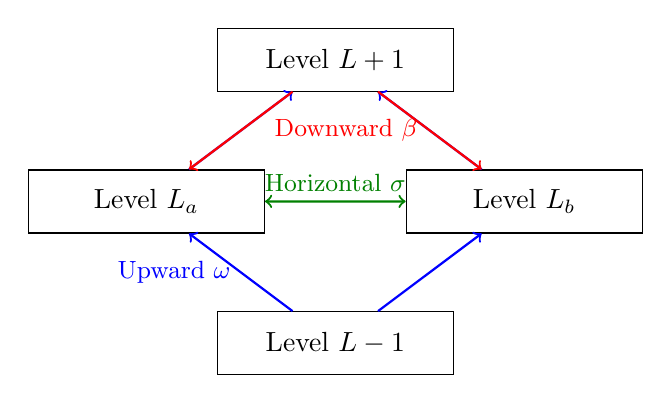
\begin{tikzpicture}[scale=1.2]
% Levels
\node[draw, rectangle, minimum width=3cm, minimum height=0.8cm] (L2) at (0,3) {Level $L+1$};
\node[draw, rectangle, minimum width=3cm, minimum height=0.8cm] (L1a) at (-2,1.5) {Level $L_a$};
\node[draw, rectangle, minimum width=3cm, minimum height=0.8cm] (L1b) at (2,1.5) {Level $L_b$};
\node[draw, rectangle, minimum width=3cm, minimum height=0.8cm] (L0) at (0,0) {Level $L-1$};

% Arrows
\draw[->, thick, blue] (L0) -- (L1a) node[midway, left] {\small Upward $\omega$};
\draw[->, thick, blue] (L0) -- (L1b);
\draw[->, thick, blue] (L1a) -- (L2);
\draw[->, thick, blue] (L1b) -- (L2);

\draw[->, thick, red] (L2) -- (L1a) node[midway, right, xshift=0.3cm] {\small Downward $\beta$};
\draw[->, thick, red] (L2) -- (L1b);

\draw[<->, thick, green!50!black] (L1a) -- (L1b) node[midway, above] {\small Horizontal $\sigma$};
\end{tikzpicture}
\caption{Three Directions of Inter-Level Dynamics}
\label{fig:aaa-three-directions}
\end{figure}

\begin{table}[htbp]
\centering
\caption{The Three Inter-Level Connections}
\label{tab:aaa-three-connections}
\renewcommand{\arraystretch}{1.4}
\begin{tabular}{@{}llll@{}}
\toprule
\textbf{Direction} & \textbf{Symbol} & \textbf{Meaning} & \textbf{Example} \\
\midrule
Upward & $\omega^L_i$ & $L-1$ aggregates to $L$ & Individuals form tribe \\
Downward & $\beta^{down}_{L}$ & $L+1$ affects $L$ & National crisis hits individuals \\
Horizontal & $\sigma_{ij}$ & Units at same $L$ interact & Tribe A affects Tribe B \\
\bottomrule
\end{tabular}
\end{table}

%%%%%%%%%%%%%%%%%%%%%%%%%%%%%%%%%%%%%%%%%%%%%%%%%%%%%%%%%%%%%%%%%%%%%%%%%%%%%%%
\section{Downward Causation}
\label{sec:aaa-downward}
%%%%%%%%%%%%%%%%%%%%%%%%%%%%%%%%%%%%%%%%%%%%%%%%%%%%%%%%%%%%%%%%%%%%%%%%%%%%%%%

\subsection{The Problem: Top-Down Effects}

Higher levels affect lower levels:
\begin{itemize}
\item National recession (L6) $\to$ Individual job loss (L0)
\item Organizational failure (L3) $\to$ Family stress (L1)
\item Tribal conflict (L2) $\to$ Individual trauma (L0)
\item Global pandemic (L8) $\to$ Everything below
\end{itemize}

This is \textbf{downward causation}---the macro affects the micro.

\subsection{Axiom AL-9: Downward Causation}

\begin{tcolorbox}[colback=gray!5!white, colframe=gray!75!black]
\textbf{Axiom AL-9: Downward Causation}
\begin{equation}
\boxed{
U^L_i = \bar{U}^L_i + \sum_{L' > L} \beta^{down}_{i,L'} \cdot U^{L'} \cdot \mathbb{1}_{i \in M^{L'}}
}
\end{equation}
where:
\begin{itemize}
\item $\beta^{down}_{i,L'}$: Sensitivity of entity $i$ at level $L$ to level $L'$
\item $\mathbb{1}_{i \in M^{L'}}$: Indicator that $i$ belongs to the higher level $L'$
\item Higher levels only affect entities that are members
\end{itemize}
\end{tcolorbox}

\subsection{Properties of Downward Causation}

\paragraph{Membership Condition.}
An entity is only affected by higher levels it belongs to:
\begin{equation}
\beta^{down}_{i,L'} > 0 \implies i \in M^{L'}
\end{equation}

A German citizen (L0) is affected by Germany (L6) but not by France (L6).

\paragraph{Distance Decay.}
Downward effects typically weaken with level distance:
\begin{equation}
|\beta^{down}_{i,L'}| \approx \beta_0 \cdot e^{-\kappa(L' - L)}
\end{equation}

Nation (L6) affects individual (L0) less directly than family (L1) does.

\paragraph{Mediation.}
Downward causation is often mediated through intermediate levels:
\begin{equation}
L+2 \to L+1 \to L \quad \text{rather than} \quad L+2 \to L \text{ directly}
\end{equation}

\subsection{The Downward Causation Matrix}

\begin{table}[htbp]
\centering
\caption{Downward Causation Coefficients $\beta^{down}$}
\label{tab:aaa-downward-matrix}
\renewcommand{\arraystretch}{1.3}
\small
\begin{tabular}{@{}l|ccccccc@{}}
\toprule
\textbf{Target $\downarrow$} & \textbf{L1} & \textbf{L2} & \textbf{L3} & \textbf{L4} & \textbf{L5} & \textbf{L6} & \textbf{L8} \\
\textbf{Source $\rightarrow$} & Family & Tribe & Org & Network & Region & Nation & Global \\
\midrule
L0 (Individual) & 0.35 & 0.28 & 0.22 & 0.10 & 0.15 & 0.18 & 0.08 \\
L1 (Family) & --- & 0.25 & 0.18 & 0.08 & 0.12 & 0.15 & 0.06 \\
L2 (Tribe) & --- & --- & 0.20 & 0.15 & 0.18 & 0.20 & 0.10 \\
L3 (Organization) & --- & --- & --- & 0.22 & 0.15 & 0.25 & 0.12 \\
L5 (Region) & --- & --- & --- & --- & --- & 0.30 & 0.15 \\
L6 (Nation) & --- & --- & --- & --- & --- & --- & 0.25 \\
\bottomrule
\end{tabular}
\begin{flushleft}
\small\textit{Note:} Coefficients show how a 1-unit change in source level affects target level.
Higher values indicate stronger downward causation.
\end{flushleft}
\end{table}

\subsection{Examples of Downward Causation}

\paragraph{Example 1: National Recession.}
\begin{align}
\Delta U^{L6}_{Nation} &= -0.3 \quad \text{(recession)} \\
\Delta U^{L0}_{Individual} &= \beta^{down}_{i,6} \cdot \Delta U^{L6} = 0.18 \times (-0.3) = -0.054
\end{align}

\paragraph{Example 2: Tribal Conflict.}
\begin{align}
\Delta U^{L2}_{Tribe} &= -0.5 \quad \text{(conflict)} \\
\Delta U^{L0}_{Individual} &= \beta^{down}_{i,2} \cdot \Delta U^{L2} = 0.28 \times (-0.5) = -0.14
\end{align}

Note: Tribal effects on individuals are stronger than national effects!

%%%%%%%%%%%%%%%%%%%%%%%%%%%%%%%%%%%%%%%%%%%%%%%%%%%%%%%%%%%%%%%%%%%%%%%%%%%%%%%
\section{Horizontal Spillover}
\label{sec:aaa-horizontal}
%%%%%%%%%%%%%%%%%%%%%%%%%%%%%%%%%%%%%%%%%%%%%%%%%%%%%%%%%%%%%%%%%%%%%%%%%%%%%%%

\subsection{The Problem: Peer Effects at Same Level}

Entities at the same level affect each other:
\begin{itemize}
\item Tribe A's success inspires Tribe B
\item Firm A's innovation pressures Firm B
\item Region A's growth attracts workers from Region B
\item Nation A's policy is copied by Nation B
\end{itemize}

This is \textbf{horizontal spillover}---peers affecting peers.

\subsection{Axiom AL-10: Horizontal Spillover}

\begin{tcolorbox}[colback=gray!5!white, colframe=gray!75!black]
\textbf{Axiom AL-10: Horizontal Spillover}
\begin{equation}
\boxed{
U^L_j = \bar{U}^L_j + \sum_{i \neq j, i \in N^L_j} \sigma^L_{ij} \cdot U^L_i
}
\end{equation}
where:
\begin{itemize}
\item $\sigma^L_{ij}$: Spillover coefficient from entity $i$ to entity $j$ at level $L$
\item $N^L_j$: Neighborhood of $j$ at level $L$ (entities that can affect $j$)
\item Spillover can be positive (cooperation) or negative (competition)
\end{itemize}
\end{tcolorbox}

\subsection{Types of Horizontal Spillover}

\begin{table}[htbp]
\centering
\caption{Types of Horizontal Spillover}
\label{tab:aaa-spillover-types}
\renewcommand{\arraystretch}{1.3}
\begin{tabular}{@{}llll@{}}
\toprule
\textbf{Type} & \textbf{$\sigma_{ij}$} & \textbf{Mechanism} & \textbf{Example} \\
\midrule
Positive/Cooperative & $> 0$ & Mutual benefit & Trade partners \\
Negative/Competitive & $< 0$ & Zero-sum rivalry & Competing firms \\
Asymmetric & $\sigma_{ij} \neq \sigma_{ji}$ & Unequal influence & Hegemon and small state \\
Network-based & $\propto$ connection & Stronger for connected & Information diffusion \\
Geographic & $\propto$ proximity & Stronger for neighbors & Regional spillovers \\
\bottomrule
\end{tabular}
\end{table}

\subsection{The Spillover Matrix at Each Level}

For each level $L$, there exists a spillover matrix $\Sigma^L$:

\begin{equation}
\Sigma^L = \begin{pmatrix}
0 & \sigma^L_{12} & \sigma^L_{13} & \cdots \\
\sigma^L_{21} & 0 & \sigma^L_{23} & \cdots \\
\sigma^L_{31} & \sigma^L_{32} & 0 & \cdots \\
\vdots & \vdots & \vdots & \ddots
\end{pmatrix}
\end{equation}

\paragraph{Properties:}
\begin{itemize}
\item Diagonal is zero (no self-spillover)
\item Generally asymmetric ($\sigma_{ij} \neq \sigma_{ji}$)
\item Sparse for large levels (not everyone affects everyone)
\end{itemize}

\subsection{Example: Tribe-Level Spillover (L2)}

Consider three neighboring tribes:

\begin{table}[htbp]
\centering
\caption{Spillover Matrix for Three Tribes}
\label{tab:aaa-tribe-spillover}
\renewcommand{\arraystretch}{1.3}
\begin{tabular}{@{}l|ccc@{}}
\toprule
$\Sigma^{L2}$ & Miners & Farmers & Merchants \\
\midrule
Miners & --- & $-0.15$ & $+0.10$ \\
Farmers & $-0.10$ & --- & $+0.20$ \\
Merchants & $+0.12$ & $+0.18$ & --- \\
\bottomrule
\end{tabular}
\end{table}

\textbf{Interpretation:}
\begin{itemize}
\item Miners-Farmers: Negative (compete for labor, environmental conflict)
\item Farmers-Merchants: Positive (trade relationship)
\item Merchants benefit from both (intermediation)
\end{itemize}

%%%%%%%%%%%%%%%%%%%%%%%%%%%%%%%%%%%%%%%%%%%%%%%%%%%%%%%%%%%%%%%%%%%%%%%%%%%%%%%
\section{The Cross-Level Complementarity Matrix}
\label{sec:aaa-cross-level-gamma}
%%%%%%%%%%%%%%%%%%%%%%%%%%%%%%%%%%%%%%%%%%%%%%%%%%%%%%%%%%%%%%%%%%%%%%%%%%%%%%%

\subsection{Beyond Within-Level Complementarity}

Section~\ref{sec:aaa-recursive} defined complementarity \emph{within} levels ($\gamma^L_{ij}$).
But there is also complementarity \emph{between} levels.

\subsection{Definition: Cross-Level Complementarity}

\begin{tcolorbox}[colback=blue!5!white, colframe=blue!50!black, title=Definition: Cross-Level Complementarity]
\begin{equation}
\boxed{
\gamma^{cross}_{L,L'} = \frac{\partial^2 U^{total}}{\partial U^L \partial U^{L'}}
}
\end{equation}

\textbf{Interpretation:}
\begin{itemize}
\item $\gamma^{cross}_{L,L'} > 0$: Levels are \textbf{complements} (reinforce each other)
\item $\gamma^{cross}_{L,L'} < 0$: Levels are \textbf{substitutes} (undermine each other)
\item $\gamma^{cross}_{L,L'} = 0$: Levels are \textbf{independent}
\end{itemize}
\end{tcolorbox}

\subsection{The Cross-Level $\Gamma^{cross}$ Matrix}

\begin{table}[htbp]
\centering
\caption{Cross-Level Complementarity Matrix $\Gamma^{cross}$}
\label{tab:aaa-cross-gamma}
\renewcommand{\arraystretch}{1.4}
\small
\begin{tabular}{@{}l|ccccccc@{}}
\toprule
$\gamma^{cross}$ & L0 & L1 & L2 & L3 & L5 & L6 & L8 \\
& Indiv. & Family & Tribe & Org & Region & Nation & Global \\
\midrule
L0 (Individual) & --- & \textbf{+0.35} & \textbf{+0.40} & +0.20 & +0.12 & +0.15 & +0.08 \\
L1 (Family) & +0.35 & --- & +0.30 & +0.10 & +0.08 & +0.10 & +0.05 \\
L2 (Tribe) & \textbf{+0.40} & +0.30 & --- & +0.25 & +0.15 & \textbf{$-$0.12} & +0.10 \\
L3 (Organization) & +0.20 & +0.10 & +0.25 & --- & +0.18 & +0.22 & +0.15 \\
L5 (Region) & +0.12 & +0.08 & +0.15 & +0.18 & --- & +0.25 & +0.12 \\
L6 (Nation) & +0.15 & +0.10 & \textbf{$-$0.12} & +0.22 & +0.25 & --- & +0.20 \\
L8 (Global) & +0.08 & +0.05 & +0.10 & +0.15 & +0.12 & +0.20 & --- \\
\bottomrule
\end{tabular}
\begin{flushleft}
\small\textit{Note:} Matrix is symmetric. Bold indicates strongest effects.
Negative values indicate structural tension between levels.
\end{flushleft}
\end{table}

\subsection{Key Findings from the Cross-Level Matrix}

\paragraph{1. Strongest Complementarity: Individual-Tribe (L0-L2).}
$$\gamma^{cross}_{0,2} = +0.40$$

Individual and tribal utility strongly reinforce each other. When the tribe
thrives, individuals thrive; when individuals succeed, the tribe benefits.
This explains the power of tribal identity.

\paragraph{2. Structural Tension: Tribe-Nation (L2-L6).}
$$\gamma^{cross}_{2,6} = -0.12$$

Tribal and national utility can \emph{conflict}. Strong tribal identity may
undermine national cohesion (separatism, sectarianism). Strong national
identity may suppress tribal identity (assimilation pressure).

\paragraph{3. Adjacent Levels Complement.}
Generally, $\gamma^{cross}_{L,L+1} > 0$. Adjacent levels tend to reinforce
each other because they share membership and direct interaction.

\paragraph{4. Distant Levels Weakly Coupled.}
$\gamma^{cross}_{L,L'}$ decreases with $|L - L'|$. Individual (L0) and Global (L8)
have weak direct complementarity ($\gamma^{cross}_{0,8} = +0.08$).

\subsection{The Tribe-Nation Tension: A Deeper Analysis}

The negative $\gamma^{cross}_{2,6}$ deserves special attention:

\begin{table}[htbp]
\centering
\caption{Tribe-Nation Tension Examples}
\label{tab:aaa-tribe-nation}
\renewcommand{\arraystretch}{1.3}
\begin{tabular}{@{}lll@{}}
\toprule
\textbf{Context} & \textbf{Manifestation} & \textbf{$\gamma^{cross}_{2,6}$} \\
\midrule
Multi-ethnic state & Ethnic groups vs. nation-building & $-0.20$ \\
Regional separatism & Catalonia, Scotland, Quebec & $-0.25$ \\
Professional tribes & ``Doctors vs. government'' & $-0.15$ \\
Religious communities & Religious law vs. secular state & $-0.18$ \\
Homogeneous nation & Tribe = Nation (Japan) & $+0.10$ \\
\bottomrule
\end{tabular}
\end{table}

\paragraph{Policy Implication.}
Policies that strengthen L6 (national identity/institutions) may weaken L2
(tribal bonds) and vice versa. Wise policy seeks configurations where both
can be positive---or explicitly manages the trade-off.

%%%%%%%%%%%%%%%%%%%%%%%%%%%%%%%%%%%%%%%%%%%%%%%%%%%%%%%%%%%%%%%%%%%%%%%%%%%%%%%
\section{Complete Inter-Level Dynamics}
\label{sec:aaa-complete-dynamics}
%%%%%%%%%%%%%%%%%%%%%%%%%%%%%%%%%%%%%%%%%%%%%%%%%%%%%%%%%%%%%%%%%%%%%%%%%%%%%%%

\subsection{The Full Dynamic Equation}

Combining all three directions (upward, downward, horizontal) plus cross-level
complementarity:

\begin{tcolorbox}[colback=green!5!white, colframe=green!50!black, title=Complete Inter-Level Utility Dynamics]
\begin{equation}
\boxed{
U^L_i(t+1) = \underbrace{\sum_{j \in M^L_i} \omega^L_j \cdot U^{L-1}_j(t)}_{\text{Upward Aggregation}}
+ \underbrace{\sum_{L' > L} \beta^{down}_{i,L'} \cdot U^{L'}(t)}_{\text{Downward Causation}}
+ \underbrace{\sum_{k \neq i} \sigma^L_{ik} \cdot U^L_k(t)}_{\text{Horizontal Spillover}}
+ \underbrace{\sum_{L' \neq L} \gamma^{cross}_{L,L'} \cdot U^{L'}(t)}_{\text{Cross-Level Complementarity}}
}
\label{eq:aaa-complete-dynamics}
\end{equation}
\end{tcolorbox}

\subsection{Matrix Form}

Let $\mathbf{U}(t) = (U^{L0}, U^{L1}, ..., U^{L8})^T$ be the vector of level utilities.

\begin{equation}
\mathbf{U}(t+1) = \mathbf{A} \cdot \mathbf{U}(t) + \mathbf{B} \cdot \mathbf{U}(t) \cdot \mathbf{U}(t)^T
\end{equation}

where:
\begin{itemize}
\item $\mathbf{A}$: Linear interaction matrix (combines $\omega$, $\beta$, $\sigma$)
\item $\mathbf{B}$: Quadratic interaction tensor (complementarities $\gamma$)
\end{itemize}

\subsection{Equilibrium Conditions}

At equilibrium, $\mathbf{U}^* = \mathbf{U}(t+1) = \mathbf{U}(t)$:

\begin{equation}
\mathbf{U}^* = \mathbf{A} \cdot \mathbf{U}^* + \mathbf{B} \cdot \mathbf{U}^* \cdot (\mathbf{U}^*)^T
\end{equation}

This is a system of nonlinear equations. Multiple equilibria are possible!

\subsection{Stability Analysis}

An equilibrium $\mathbf{U}^*$ is stable if small perturbations decay:

\begin{equation}
\left| \frac{\partial U^L_i(t+1)}{\partial U^{L'}_j(t)} \right|_{\mathbf{U}^*} < 1 \quad \forall L, L', i, j
\end{equation}

\paragraph{Stability Conditions:}
\begin{itemize}
\item Strong positive cross-level complementarity $\to$ Multiple stable equilibria
\item Strong negative cross-level complementarity $\to$ Oscillations, instability
\item Balanced complementarity $\to$ Unique stable equilibrium
\end{itemize}

%%%%%%%%%%%%%%%%%%%%%%%%%%%%%%%%%%%%%%%%%%%%%%%%%%%%%%%%%%%%%%%%%%%%%%%%%%%%%%%
\section{Implications for EBF Practice}
\label{sec:aaa-implications}
%%%%%%%%%%%%%%%%%%%%%%%%%%%%%%%%%%%%%%%%%%%%%%%%%%%%%%%%%%%%%%%%%%%%%%%%%%%%%%%

\subsection{Intervention Design}

\begin{table}[htbp]
\centering
\caption{Inter-Level Considerations for Interventions}
\label{tab:aaa-intervention-implications}
\renewcommand{\arraystretch}{1.3}
\begin{tabular}{@{}lll@{}}
\toprule
\textbf{Question} & \textbf{Relevant Dynamic} & \textbf{Consideration} \\
\midrule
Where to intervene? & Cross-level $\gamma$ & Target level with highest spillover \\
Will it scale? & Horizontal $\sigma$ & Check if positive spillover exists \\
Unintended consequences? & Downward $\beta$ & Higher-level effects cascade down \\
Sustainability? & Equilibrium stability & Is new state stable? \\
Trade-offs? & Negative $\gamma^{cross}$ & Improving L may hurt L' \\
\bottomrule
\end{tabular}
\end{table}

\subsection{Why Interventions Fail: An Inter-Level Analysis}

\paragraph{Failure Mode 1: Ignoring Downward Effects.}
Intervention at L0 (individual training) fails because L2 (tribe) or L6 (nation)
creates opposing pressure via $\beta^{down}$.

\textit{Example: Individual job training fails because tribal identity (``we don't do that'')
exerts downward pressure.}

\paragraph{Failure Mode 2: Negative Horizontal Spillover.}
Success at one unit triggers negative spillover to peers.

\textit{Example: One firm's green transition triggers competitive response from rivals,
negating aggregate benefit.}

\paragraph{Failure Mode 3: Cross-Level Substitution.}
Strengthening one level weakens another due to $\gamma^{cross} < 0$.

\textit{Example: National integration policy strengthens L6 but weakens L2 (tribal identity),
creating backlash.}

\paragraph{Failure Mode 4: Unstable Equilibrium.}
New state is not an equilibrium; system reverts.

\textit{Example: Temporary behavior change reverts when intervention stops because
underlying level structure unchanged.}

\subsection{Success Conditions}

For sustainable behavioral change:

\begin{tcolorbox}[colback=green!5!white, colframe=green!50!black, title=Conditions for Successful Multi-Level Intervention]
\begin{enumerate}
\item \textbf{Level Alignment:} $\gamma^{cross}_{L,L'} > 0$ for all affected levels
\item \textbf{Positive Spillover:} $\sum_j \sigma_{ij} \geq 0$ (peers support change)
\item \textbf{Downward Support:} $\beta^{down} \cdot \Delta U^{L+1} \geq 0$ (higher levels support)
\item \textbf{Stable Equilibrium:} New configuration is dynamically stable
\end{enumerate}
\end{tcolorbox}

%%%%%%%%%%%%%%%%%%%%%%%%%%%%%%%%%%%%%%%%%%%%%%%%%%%%%%%%%%%%%%%%%%%%%%%%%%%%%%%
\section{Extended Coal Miner Example}
\label{sec:aaa-extended-miner}
%%%%%%%%%%%%%%%%%%%%%%%%%%%%%%%%%%%%%%%%%%%%%%%%%%%%%%%%%%%%%%%%%%%%%%%%%%%%%%%

\subsection{The Inter-Level Analysis}

Revisiting the coal miner with full inter-level dynamics:

\paragraph{Upward Effects (miner retrains):}
\begin{itemize}
\item L0 $\to$ L1: Family benefits ($\omega > 0$, positive)
\item L0 $\to$ L2: Tribe loses member ($\omega > 0$, but contribution negative)
\end{itemize}

\paragraph{Downward Effects:}
\begin{itemize}
\item L2 $\to$ L0: Tribal disapproval ($\beta^{down}_{miner,2} = 0.28$, negative)
\item L5 $\to$ L0: Regional decline ($\beta^{down}_{miner,5} = 0.15$, negative)
\end{itemize}

\paragraph{Horizontal Spillover (if miner retrains):}
\begin{itemize}
\item Other miners see possibility ($\sigma > 0$) OR
\item Other miners feel betrayed ($\sigma < 0$)
\end{itemize}

\paragraph{Cross-Level Complementarity:}
\begin{itemize}
\item L0-L2: $\gamma^{cross}_{0,2} = +0.40$ means individual and tribal utility
are tightly linked---hard to improve one without the other
\end{itemize}

\subsection{Why Individual Retraining Fails}

\begin{equation}
\Delta U^{total} = \underbrace{\Delta U^{L0}_{INU}}_{\text{+income}} 
+ \underbrace{\gamma^{cross}_{0,2} \cdot \Delta U^{L2}}_{\text{tribal loss } \times 0.40}
+ \underbrace{\beta^{down}_{0,2} \cdot \Delta U^{L2}}_{\text{downward pressure}}
\end{equation}

Even if $\Delta U^{L0}_{INU} > 0$, the tribal effects dominate because:
\begin{itemize}
\item $\gamma^{cross}_{0,2} = +0.40$ (strong coupling)
\item $\beta^{down}_{0,2} = 0.28$ (strong downward effect)
\item $\Delta U^{L2} < 0$ (tribal utility falls)
\end{itemize}

\subsection{Successful Intervention: Collective Transition}

Move the tribe together:

\begin{equation}
\Delta U^{L2} > 0 \implies \begin{cases}
\gamma^{cross}_{0,2} \cdot \Delta U^{L2} > 0 & \text{(cross-level positive)} \\
\beta^{down}_{0,2} \cdot \Delta U^{L2} > 0 & \text{(downward positive)} \\
\sigma_{ij} \cdot \Delta U^{L2}_i > 0 & \text{(horizontal positive)}
\end{cases}
\end{equation}

All inter-level effects align positively when the tribe transitions together.

%%%%%%%%%%%%%%%%%%%%%%%%%%%%%%%%%%%%%%%%%%%%%%%%%%%%%%%%%%%%%%%%%%%%%%%%%%%%%%%
\section{Summary: Inter-Level Dynamics}
\label{sec:aaa-inter-level-summary}
%%%%%%%%%%%%%%%%%%%%%%%%%%%%%%%%%%%%%%%%%%%%%%%%%%%%%%%%%%%%%%%%%%%%%%%%%%%%%%%

\begin{tcolorbox}[colback=gray!5!white, colframe=gray!75!black, title=Inter-Level Dynamics Summary]

\textbf{Three Directions:}
\begin{itemize}
\item Upward Aggregation: $U^L = \sum \omega_i U^{L-1}_i$ (AL-3)
\item Downward Causation: $\Delta U^L = \beta^{down} \cdot \Delta U^{L+1}$ (AL-9)
\item Horizontal Spillover: $U^L_j = f(\sigma_{ij} \cdot U^L_i)$ (AL-10)
\end{itemize}

\textbf{Cross-Level Complementarity:}
$$\gamma^{cross}_{L,L'} = \frac{\partial^2 U^{total}}{\partial U^L \partial U^{L'}}$$

\textbf{Key Finding:}
Individual-Tribe ($\gamma^{cross}_{0,2} = +0.40$) is the strongest cross-level link.

\textbf{Structural Tension:}
Tribe-Nation ($\gamma^{cross}_{2,6} = -0.12$) can conflict.

\textbf{Complete Dynamics:}
$$U^L(t+1) = \text{Upward} + \text{Downward} + \text{Horizontal} + \text{Cross-Level}$$

\textbf{Intervention Implication:}
Sustainable change requires alignment across all inter-level effects.

\end{tcolorbox}

%%%%%%%%%%%%%%%%%%%%%%%%%%%%%%%%%%%%%%%%%%%%%%%%%%%%%%%%%%%%%%%%%%%%%%%%%%%%%%%
\section{Extended Glossary: Inter-Level Symbols}
\label{sec:aaa-extended-glossary}
%%%%%%%%%%%%%%%%%%%%%%%%%%%%%%%%%%%%%%%%%%%%%%%%%%%%%%%%%%%%%%%%%%%%%%%%%%%%%%%

\begin{table}[htbp]
\centering
\caption{Additional Symbols for Inter-Level Dynamics}
\label{tab:aaa-extended-symbols}
\renewcommand{\arraystretch}{1.3}
\begin{tabular}{@{}lll@{}}
\toprule
\textbf{Symbol} & \textbf{Name} & \textbf{Definition} \\
\midrule
$\beta^{down}_{i,L'}$ & Downward coefficient & Effect of level $L'$ on entity $i$ at lower level \\
$\sigma^L_{ij}$ & Spillover coefficient & Effect of entity $i$ on entity $j$ at same level $L$ \\
$\Sigma^L$ & Spillover matrix & Matrix of $\sigma^L_{ij}$ for level $L$ \\
$\gamma^{cross}_{L,L'}$ & Cross-level complementarity & Interaction between levels $L$ and $L'$ \\
$\Gamma^{cross}$ & Cross-level matrix & Matrix of all $\gamma^{cross}_{L,L'}$ \\
$N^L_j$ & Neighborhood & Entities that can affect $j$ at level $L$ \\
$\kappa$ & Distance decay & Rate of decay with level distance \\
$\mathbf{A}$ & Linear interaction matrix & Combined upward, downward, horizontal effects \\
$\mathbf{B}$ & Quadratic interaction tensor & Complementarity effects \\
$\mathbf{U}^*$ & Equilibrium & Stable configuration of level utilities \\
\bottomrule
\end{tabular}
\end{table}

%%%%%%%%%%%%%%%%%%%%%%%%%%%%%%%%%%%%%%%%%%%%%%%%%%%%%%%%%%%%%%%%%%%%%%%%%%%%%%%
% END OF APPENDIX AAA
%%%%%%%%%%%%%%%%%%%%%%%%%%%%%%%%%%%%%%%%%%%%%%%%%%%%%%%%%%%%%%%%%%%%%%%%%%%%%%%
%%%%%%%%%%%%%%%%%%%%%%%%%%%%%%%%%%%%%%%%%%%%%%%%%%%%%%%%%%%%%%%%%%%%%%%%%%%%%%%
%%%%%%%%%%%%%%%%%%%%%%%%%%%%%%%%%%%%%%%%%%%%%%%%%%%%%%%%%%%%%%%%%%%%%%%%%%%%%%%
%%%%%%%%%%%%%%%%%%%%%%%%%%%%%%%%%%%%%%%%%%%%%%%%%%%%%%%%%%%%%%%%%%%%%%%%%%%%%%%
%%
%%  THE GENERAL THEORY OF WELFARE HIERARCHIES (GTWH)
%%
%%  A Unified Framework for Multi-Level Welfare Analysis
%%
%%%%%%%%%%%%%%%%%%%%%%%%%%%%%%%%%%%%%%%%%%%%%%%%%%%%%%%%%%%%%%%%%%%%%%%%%%%%%%%
%%%%%%%%%%%%%%%%%%%%%%%%%%%%%%%%%%%%%%%%%%%%%%%%%%%%%%%%%%%%%%%%%%%%%%%%%%%%%%%

\section{The General Theory of Welfare Hierarchies}
\label{sec:gtwh}

\begin{center}
\Large\textbf{The General Theory of Welfare Hierarchies (GTWH)}\\[0.5em]
\large\textit{A Unified Framework for Multi-Level Welfare Analysis}\\[1em]
\normalsize
Gerhard Fehr\\
FehrAdvice \& Partners AG, Zürich\\[0.5em]
January 2026
\end{center}

\vspace{1em}

\begin{abstract}
We present the \textbf{General Theory of Welfare Hierarchies (GTWH)}, a unified 
framework that resolves the fundamental aggregation problem in welfare economics. 
The theory derives the complete structure of social levels---from individual to 
humanity---from first principles, showing that levels are \emph{endogenously 
defined} by shared identity (IDN) and collective utility (KNU) rather than 
exogenously assumed. The framework features: (1) a recursive, self-similar 
utility structure that applies identically at every level; (2) three formally 
specified inter-level dynamics (upward aggregation, downward causation, 
horizontal spillover); (3) a cross-level complementarity matrix capturing 
how levels reinforce or undermine each other; and (4) context-dependent 
level salience determined by the environment. The theory unifies methodological 
individualism with holistic approaches, bridges micro and macro analysis, 
and provides a rigorous foundation for welfare economics, social choice theory, 
and policy design across all scales of human organization.
\end{abstract}

\vspace{1em}
\noindent\textbf{Keywords:} Welfare economics, aggregation problem, multi-level 
analysis, social hierarchy, utility theory, complementarity, identity economics

\noindent\textbf{JEL Classification:} D60, D71, D91, Z13

%%%%%%%%%%%%%%%%%%%%%%%%%%%%%%%%%%%%%%%%%%%%%%%%%%%%%%%%%%%%%%%%%%%%%%%%%%%%%%%
\subsection{Introduction: The Aggregation Problem}
%%%%%%%%%%%%%%%%%%%%%%%%%%%%%%%%%%%%%%%%%%%%%%%%%%%%%%%%%%%%%%%%%%%%%%%%%%%%%%%

\paragraph{The Central Problem of Welfare Economics.}
Since Arrow's (1951) impossibility theorem, welfare economics has struggled 
with a fundamental question: \textit{How do individual utilities aggregate to 
social welfare?} The problem is not merely technical but conceptual:

\begin{itemize}
\item What is the relationship between individual and collective welfare?
\item Do groups, organizations, and nations have welfare beyond their members?
\item How do we compare welfare across different levels of social organization?
\item Why do policies that help individuals sometimes harm communities, and vice versa?
\end{itemize}

\paragraph{The Limitations of Existing Approaches.}
Current approaches fall into two camps, each with fundamental limitations:

\begin{enumerate}
\item \textbf{Methodological Individualism}: Only individuals have utility; 
social welfare is merely the sum of individual utilities. 
\textit{Problem}: Cannot explain why tribal identity affects behavior, 
why national institutions matter, or why communities have emergent properties.

\item \textbf{Holistic Approaches}: Groups have irreducible properties that 
cannot be explained by individual behavior.
\textit{Problem}: No micro-foundation; cannot explain how group properties 
emerge from individual actions.
\end{enumerate}

\paragraph{The GTWH Resolution.}
The General Theory of Welfare Hierarchies resolves this tension by showing that:
\begin{enumerate}
\item Levels are \textbf{endogenously defined} by shared identity and collective structure
\item The \textbf{same utility formula} applies at every level (self-similarity)
\item Levels \textbf{interact dynamically} through upward, downward, and horizontal connections
\item Level \textbf{salience depends on context}, explaining situational variation
\item The framework \textbf{converges} to a well-defined meta-level (all sentient beings)
\end{enumerate}

%%%%%%%%%%%%%%%%%%%%%%%%%%%%%%%%%%%%%%%%%%%%%%%%%%%%%%%%%%%%%%%%%%%%%%%%%%%%%%%
\subsection{The Core Insight: Endogenous Levels}
%%%%%%%%%%%%%%%%%%%%%%%%%%%%%%%%%%%%%%%%%%%%%%%%%%%%%%%%%%%%%%%%%%%%%%%%%%%%%%%

\paragraph{The Conventional View.}
Standard economics assumes levels exist exogenously:
\begin{itemize}
\item Microeconomics: Individuals and firms (given)
\item Macroeconomics: Nations and economies (given)
\item International economics: Countries (given)
\end{itemize}

The levels are simply \textit{assumed}, not derived.

\paragraph{The GTWH Innovation.}
We reverse the logic. Instead of assuming levels and asking how they interact, 
we ask: \textit{What defines a level?}

\begin{tcolorbox}[colback=blue!5!white, colframe=blue!75!black, title=The Endogeneity Principle]
\textbf{A level exists if and only if there is shared identity (IDN) or 
shared collective utility (KNU).}

\begin{equation}
\boxed{
\text{Level } L \text{ exists} \iff \exists \, IDN^L \text{ (shared identity)} \lor \exists \, KNU^L \text{ (shared collective)}
}
\end{equation}

Levels are not given---they are \textbf{created} by human identification and cooperation.
\end{tcolorbox}

\paragraph{Implications.}
\begin{itemize}
\item \textbf{Levels can emerge}: When people form a shared identity (``We are X''), 
a new level comes into existence.
\item \textbf{Levels can dissolve}: When identity fades or collectives fragment, 
levels disappear.
\item \textbf{Levels are context-dependent}: The same person belongs to multiple 
levels; which is salient depends on context.
\item \textbf{Levels are empirically identifiable}: Wherever we find shared 
identity or collective structure, there is a level.
\end{itemize}

%%%%%%%%%%%%%%%%%%%%%%%%%%%%%%%%%%%%%%%%%%%%%%%%%%%%%%%%%%%%%%%%%%%%%%%%%%%%%%%
\subsection{The Foundational Structure}
%%%%%%%%%%%%%%%%%%%%%%%%%%%%%%%%%%%%%%%%%%%%%%%%%%%%%%%%%%%%%%%%%%%%%%%%%%%%%%%

\subsubsection{The Meta Level: The Ultimate Scope}

\paragraph{The Foundational Question.}
Before deriving levels, we must answer: \textit{What is the ultimate scope of 
welfare analysis?}

\paragraph{The Sentience Criterion.}
Following Nagel (1974), Chalmers (1996), and Singer (1975), we adopt the principle 
that welfare requires a \textit{subject of experience}---an entity for which there 
is ``something it is like'' to be that entity. Chalmers' formulation of the 
``hard problem of consciousness'' provides the philosophical foundation: subjective 
experience (qualia) cannot be reduced to functional or physical descriptions, yet 
it is precisely this subjective dimension that makes welfare possible. An entity 
without phenomenal consciousness---without ``something it is like'' to be that 
entity---cannot have welfare in any meaningful sense.

\begin{tcolorbox}[colback=green!5!white, colframe=green!50!black, title=Definition: The Meta Level]
\begin{equation}
\boxed{
U^{Meta} = \int_{t=0}^{\infty} \sum_{i \in S_t} \delta^t \cdot U^i_t \, dt
}
\end{equation}

where $S_t$ is the set of all sentient beings at time $t$, and $\delta$ is the 
intergenerational discount factor.

The Meta level encompasses \textbf{all welfare that exists or will exist}.
\end{tcolorbox}

\paragraph{Philosophical Grounding.}
This formulation:
\begin{itemize}
\item Includes all humans (present and future)
\item Includes sentient animals (per Singer's expanding circle)
\item Potentially includes future artificial sentience
\item Provides a well-defined upper bound for the hierarchy
\end{itemize}

\subsubsection{The Recursive Structure}

\paragraph{The Self-Similarity Principle.}
A remarkable feature of welfare hierarchies is their \textit{self-similarity}: 
the same mathematical structure applies at every level.

\begin{tcolorbox}[colback=yellow!5!white, colframe=yellow!50!black, title=The Recursive Welfare Formula]
At \textbf{any} level $L$:

\begin{equation}
\boxed{
U^L_{d,t}(\Psi) = \left(\delta^L_d(\Psi)\right)^t \cdot \left[ G^L_{d,t} - \lambda^L_d(\Psi) \cdot P^L_{d,t} \right]
}
\end{equation}

\textbf{Aggregation} from level $L-1$ to level $L$:

\begin{equation}
\boxed{
U^L = \sum_{i \in M^L} \omega^L_i \cdot U^{L-1}_i + \sum_{i < j} \gamma^L_{ij} \cdot U^{L-1}_i \cdot U^{L-1}_j
}
\end{equation}

The formula is \textbf{fractal}: zoom in or out, and you see the same structure.
\end{tcolorbox}

\paragraph{Why Self-Similarity?}
The self-similar structure is not arbitrary. It reflects:
\begin{itemize}
\item \textbf{Prospect theory} (Kahneman \& Tversky, 1979): Gain-loss asymmetry 
operates at all levels---individuals fear losses, so do organizations and nations.
\item \textbf{Discounting} (Samuelson, 1937): All entities discount the future, 
whether persons, firms, or governments.
\item \textbf{Complementarity} (Milgrom \& Roberts, 1990): Interaction effects 
exist at every level of organization.
\end{itemize}

%%%%%%%%%%%%%%%%%%%%%%%%%%%%%%%%%%%%%%%%%%%%%%%%%%%%%%%%%%%%%%%%%%%%%%%%%%%%%%%
\subsection{The Level Hierarchy}
%%%%%%%%%%%%%%%%%%%%%%%%%%%%%%%%%%%%%%%%%%%%%%%%%%%%%%%%%%%%%%%%%%%%%%%%%%%%%%%

\paragraph{Derived Levels.}
Applying the endogeneity principle, we derive the following hierarchy:

\begin{table}[htbp]
\centering
\caption{The GTWH Level Hierarchy}
\label{tab:gtwh-hierarchy}
\renewcommand{\arraystretch}{1.4}
\begin{tabular}{@{}clll@{}}
\toprule
$L$ & \textbf{Level} & \textbf{Defining Condition} & \textbf{Examples} \\
\midrule
0 & Individual & Sentience (base case) & A person \\
1 & Primary Group & Kinship, strong bonds & Family, close friends \\
2 & Tribe/Community & Shared identity ``We are X'' & Profession, village, clan \\
3 & Organization & Formal collective structure & Firm, party, church \\
4 & Network & Functional interdependence & Industry, movement \\
5 & Region & Geographic collective & City, state, canton \\
6 & Nation & Political collective & Country \\
7 & Supranational & Treaty-based collective & EU, ASEAN \\
8 & Species & Biological identity & Humanity \\
9 & Sentient & Consciousness & All sentient beings \\
$\infty$ & Meta & Intertemporal & All sentient, all time \\
\bottomrule
\end{tabular}
\end{table}

\paragraph{The Critical Role of Level 2 (Tribe).}
Empirically, Level 2 (Tribe/Community) has outsized importance:
\begin{itemize}
\item Strongest identity effects (``We are miners'' often > ``We are Americans'')
\item Dunbar's number (~150) suggests cognitive optimization for this scale
\item Most behavioral interventions succeed or fail at this level
\item Explains resistance to individually beneficial changes (coal miner retraining)
\end{itemize}

%%%%%%%%%%%%%%%%%%%%%%%%%%%%%%%%%%%%%%%%%%%%%%%%%%%%%%%%%%%%%%%%%%%%%%%%%%%%%%%
\subsection{Inter-Level Dynamics: The Three Connections}
%%%%%%%%%%%%%%%%%%%%%%%%%%%%%%%%%%%%%%%%%%%%%%%%%%%%%%%%%%%%%%%%%%%%%%%%%%%%%%%

\paragraph{Beyond Static Aggregation.}
Levels do not exist in isolation. They are connected by three dynamic processes:

\begin{figure}[htbp]
\centering
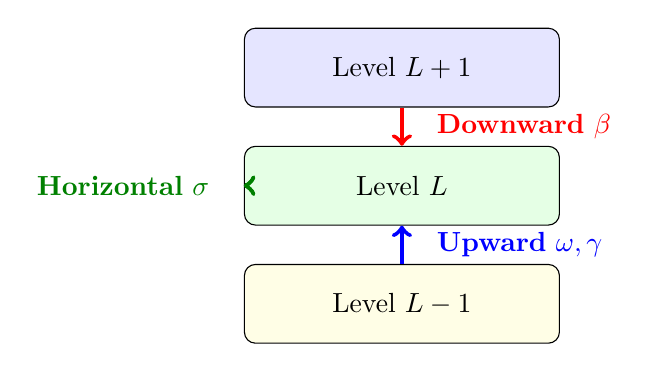
\begin{tikzpicture}[scale=1.0]
% Levels
\node[draw, rectangle, rounded corners, minimum width=4cm, minimum height=1cm, fill=blue!10] (Lplus) at (0,3) {Level $L+1$};
\node[draw, rectangle, rounded corners, minimum width=4cm, minimum height=1cm, fill=green!10] (L) at (0,1.5) {Level $L$};
\node[draw, rectangle, rounded corners, minimum width=4cm, minimum height=1cm, fill=yellow!10] (Lminus) at (0,0) {Level $L-1$};

% Arrows
\draw[->, ultra thick, blue] (Lminus.north) -- (L.south) 
    node[midway, right, xshift=0.3cm] {\textbf{Upward} $\omega, \gamma$};
\draw[->, ultra thick, red] (Lplus.south) -- (L.north) 
    node[midway, right, xshift=0.3cm] {\textbf{Downward} $\beta$};
\draw[<->, ultra thick, green!50!black] (L.west) .. controls (-2,1.5) and (-2,1.5) .. (L.west)
    node[midway, left, xshift=-0.3cm] {\textbf{Horizontal} $\sigma$};
\end{tikzpicture}
\caption{The Three Inter-Level Connections}
\label{fig:gtwh-connections}
\end{figure}

\subsubsection{Upward Aggregation}

\begin{equation}
U^L = \sum_{i} \omega^L_i \cdot U^{L-1}_i + \sum_{i < j} \gamma^L_{ij} \cdot U^{L-1}_i \cdot U^{L-1}_j
\end{equation}

Lower-level utilities aggregate to higher levels, with complementarities.

\textit{Example}: Individual workers' utilities aggregate to firm welfare, 
but with interaction effects---a team of complementary skills produces more 
than the sum of individual contributions.

\subsubsection{Downward Causation}

\begin{equation}
U^L_i = \bar{U}^L_i + \sum_{L' > L} \beta^{down}_{i,L'} \cdot U^{L'} \cdot \mathbb{1}_{i \in M^{L'}}
\end{equation}

Higher-level states causally affect lower levels.

\textit{Example}: A national recession (L6) causes individual job losses (L0). 
The macro affects the micro.

\subsubsection{Horizontal Spillover}

\begin{equation}
U^L_j = \bar{U}^L_j + \sum_{i \neq j} \sigma^L_{ij} \cdot U^L_i
\end{equation}

Entities at the same level affect each other.

\textit{Example}: One tribe's success inspires neighboring tribes (positive spillover); 
one firm's innovation pressures competitors (negative spillover).

%%%%%%%%%%%%%%%%%%%%%%%%%%%%%%%%%%%%%%%%%%%%%%%%%%%%%%%%%%%%%%%%%%%%%%%%%%%%%%%
\subsection{The Cross-Level Complementarity Matrix}
%%%%%%%%%%%%%%%%%%%%%%%%%%%%%%%%%%%%%%%%%%%%%%%%%%%%%%%%%%%%%%%%%%%%%%%%%%%%%%%

\paragraph{Beyond Additive Aggregation.}
A key innovation of GTWH is recognizing that levels themselves are 
\textit{complements or substitutes}:

\begin{equation}
\gamma^{cross}_{L,L'} = \frac{\partial^2 U^{total}}{\partial U^L \partial U^{L'}}
\end{equation}

\begin{table}[htbp]
\centering
\caption{Cross-Level Complementarity Matrix $\Gamma^{cross}$ (Key Values)}
\label{tab:gtwh-gamma-cross}
\renewcommand{\arraystretch}{1.3}
\begin{tabular}{@{}lccccc@{}}
\toprule
& L0 (Indiv.) & L1 (Family) & L2 (Tribe) & L6 (Nation) & L8 (Global) \\
\midrule
L0 (Individual) & --- & +0.35 & \textbf{+0.40} & +0.15 & +0.08 \\
L2 (Tribe) & \textbf{+0.40} & +0.30 & --- & \textbf{--0.12} & +0.10 \\
L6 (Nation) & +0.15 & +0.10 & \textbf{--0.12} & --- & +0.20 \\
\bottomrule
\end{tabular}
\end{table}

\paragraph{Key Findings.}
\begin{enumerate}
\item \textbf{Individual-Tribe Complementarity} ($\gamma^{cross}_{0,2} = +0.40$): 
The strongest cross-level link. When tribes thrive, individuals thrive. 
This explains the power of community.

\item \textbf{Tribe-Nation Tension} ($\gamma^{cross}_{2,6} = -0.12$): 
Tribal and national welfare can \textit{conflict}. Strong tribal identity 
may undermine national cohesion (separatism); strong national identity 
may suppress tribal identity (forced assimilation).

\item \textbf{Adjacent Complementarity}: Generally, $\gamma^{cross}_{L,L+1} > 0$. 
Adjacent levels tend to reinforce each other.

\item \textbf{Distance Decay}: $|\gamma^{cross}_{L,L'}|$ decreases with $|L - L'|$. 
Distant levels interact weakly.
\end{enumerate}

%%%%%%%%%%%%%%%%%%%%%%%%%%%%%%%%%%%%%%%%%%%%%%%%%%%%%%%%%%%%%%%%%%%%%%%%%%%%%%%
\subsection{Context and Level Salience}
%%%%%%%%%%%%%%%%%%%%%%%%%%%%%%%%%%%%%%%%%%%%%%%%%%%%%%%%%%%%%%%%%%%%%%%%%%%%%%%

\paragraph{The Salience Problem.}
A person simultaneously belongs to multiple levels (individual, family member, 
professional, citizen, human). Which level ``matters'' at any moment?

\begin{equation}
L^*(\Psi) = \arg\max_L \left[ A^L(\Psi) \right]
\end{equation}

Context $\Psi$ determines level salience.

\paragraph{Context Effects.}
\begin{table}[htbp]
\centering
\caption{Context Triggers for Level Salience}
\label{tab:gtwh-salience}
\renewcommand{\arraystretch}{1.3}
\begin{tabular}{@{}lll@{}}
\toprule
\textbf{Context} & \textbf{Salient Level} & \textbf{Example} \\
\midrule
Personal crisis & L0 (Individual) & Health diagnosis \\
Family event & L1 (Primary) & Wedding, funeral \\
Professional setting & L2 (Tribe) & Industry conference \\
Organizational context & L3 (Organization) & Company meeting \\
National event & L6 (Nation) & World Cup, election \\
Existential threat & L8+ (Species) & Pandemic, climate crisis \\
\bottomrule
\end{tabular}
\end{table}

\paragraph{Policy Implication.}
Effective policy must activate the \textit{right level}. Climate policy 
fails when it activates L6 (national interest) instead of L8 (species survival). 
Retraining programs fail when they activate L0 (individual benefit) but 
ignore L2 (tribal identity loss).

%%%%%%%%%%%%%%%%%%%%%%%%%%%%%%%%%%%%%%%%%%%%%%%%%%%%%%%%%%%%%%%%%%%%%%%%%%%%%%%
\subsection{The Complete Dynamic System}
%%%%%%%%%%%%%%%%%%%%%%%%%%%%%%%%%%%%%%%%%%%%%%%%%%%%%%%%%%%%%%%%%%%%%%%%%%%%%%%

\paragraph{Full Specification.}
Combining all elements, the complete GTWH dynamic is:

\begin{tcolorbox}[colback=blue!5!white, colframe=blue!75!black, title=The GTWH Master Equation]
\begin{equation}
\boxed{
U^L_i(t+1) = \underbrace{\sum_{j} \omega^L_{ij} U^{L-1}_j(t)}_{\text{Upward}} + 
\underbrace{\sum_{L'>L} \beta^{down}_{i,L'} U^{L'}(t)}_{\text{Downward}} + 
\underbrace{\sum_{k \neq i} \sigma^L_{ik} U^L_k(t)}_{\text{Horizontal}} + 
\underbrace{\sum_{L' \neq L} \gamma^{cross}_{L,L'} U^{L'}(t)}_{\text{Cross-Level}}
}
\end{equation}
\end{tcolorbox}

\paragraph{Matrix Form.}
\begin{equation}
\mathbf{U}(t+1) = \mathbf{A} \cdot \mathbf{U}(t) + \mathbf{U}(t)^\top \cdot \mathbf{B} \cdot \mathbf{U}(t)
\end{equation}

where $\mathbf{A}$ captures linear effects (upward, downward, horizontal) and 
$\mathbf{B}$ captures quadratic effects (complementarities).

\paragraph{Equilibrium.}
The system has equilibrium $\mathbf{U}^*$ satisfying:
\begin{equation}
\mathbf{U}^* = \mathbf{A} \cdot \mathbf{U}^* + (\mathbf{U}^*)^\top \cdot \mathbf{B} \cdot \mathbf{U}^*
\end{equation}

Stability requires the spectral radius $\rho(\mathbf{A}) < 1$.

%%%%%%%%%%%%%%%%%%%%%%%%%%%%%%%%%%%%%%%%%%%%%%%%%%%%%%%%%%%%%%%%%%%%%%%%%%%%%%%
\subsection{Theoretical Contributions}
%%%%%%%%%%%%%%%%%%%%%%%%%%%%%%%%%%%%%%%%%%%%%%%%%%%%%%%%%%%%%%%%%%%%%%%%%%%%%%%

\paragraph{GTWH makes five fundamental contributions:}

\begin{enumerate}
\item \textbf{Resolves the Micro-Macro Problem}

The longstanding divide between methodological individualism and holism is 
resolved: levels emerge from individual identity and cooperation (micro-foundation), 
but once emerged, they have causal power over individuals (macro-effect). 
Both perspectives are correct---at different points in the causal chain.

\item \textbf{Provides a Complete Aggregation Theory}

Unlike Arrow's impossibility result (which shows aggregation of preferences 
is problematic), GTWH shows aggregation of \textit{welfare} is well-defined 
when complementarities are included. The key is the interaction term 
$\sum \gamma_{ij} U_i U_j$.

\item \textbf{Explains Cross-Level Conflicts}

Why do individually beneficial policies sometimes harm communities? 
Why does national cohesion sometimes require suppressing local identities? 
GTWH explains these through the $\Gamma^{cross}$ matrix: some level pairs 
are substitutes ($\gamma^{cross} < 0$), creating inherent tension.

\item \textbf{Unifies Welfare Economics with Identity Economics}

Previous frameworks (Akerlof \& Kranton, 2000) add identity to individual 
utility. GTWH goes further: identity \textit{defines} levels. IDN is not 
just a component of utility---it is the mechanism by which social structure exists.

\item \textbf{Establishes a Meta-Ethical Foundation}

By grounding the hierarchy in sentience, GTWH provides a philosophically 
defensible answer to ``whose welfare counts?''---all beings capable of 
subjective experience, across all time.

\end{enumerate}

%%%%%%%%%%%%%%%%%%%%%%%%%%%%%%%%%%%%%%%%%%%%%%%%%%%%%%%%%%%%%%%%%%%%%%%%%%%%%%%
\subsection{Empirical Implications}
%%%%%%%%%%%%%%%%%%%%%%%%%%%%%%%%%%%%%%%%%%%%%%%%%%%%%%%%%%%%%%%%%%%%%%%%%%%%%%%

\paragraph{The theory generates testable predictions:}

\begin{enumerate}
\item \textbf{Tribe-Level Dominance}: Interventions addressing L2 (tribal identity) 
will be more effective than those addressing only L0 (individual incentives).
\textit{Test}: Compare retraining programs with vs. without community components.

\item \textbf{Cross-Level Trade-offs}: Policies strengthening L6 (national institutions) 
will weaken L2 (tribal bonds) in contexts with negative $\gamma^{cross}_{2,6}$.
\textit{Test}: Measure tribal identity before/after nation-building policies.

\item \textbf{Context-Dependent Salience}: Framing the same choice at different 
levels will produce different decisions.
\textit{Test}: Frame climate action as individual (L0), community (L2), or 
species (L8) issue; measure behavioral response.

\item \textbf{Downward Causation Magnitude}: $\beta^{down}$ coefficients 
should decay with level distance.
\textit{Test}: Measure individual welfare response to shocks at different levels.

\item \textbf{Spillover Asymmetry}: Positive and negative spillovers ($\sigma$) 
should have different magnitudes (loss aversion applies to spillovers).
\textit{Test}: Compare magnitude of competitive vs. cooperative peer effects.
\end{enumerate}

%%%%%%%%%%%%%%%%%%%%%%%%%%%%%%%%%%%%%%%%%%%%%%%%%%%%%%%%%%%%%%%%%%%%%%%%%%%%%%%
\subsection{Policy Applications}
%%%%%%%%%%%%%%%%%%%%%%%%%%%%%%%%%%%%%%%%%%%%%%%%%%%%%%%%%%%%%%%%%%%%%%%%%%%%%%%

\paragraph{GTWH provides a framework for policy design:}

\begin{table}[htbp]
\centering
\caption{Policy Design Principles from GTWH}
\label{tab:gtwh-policy}
\renewcommand{\arraystretch}{1.4}
\begin{tabular}{@{}p{4cm}p{5cm}p{5cm}@{}}
\toprule
\textbf{Principle} & \textbf{Implication} & \textbf{Example} \\
\midrule
Target the right level & Identify which level is salient for the behavior & Climate: Activate L8, not L6 \\
Address cross-level tensions & Anticipate $\gamma^{cross} < 0$ conflicts & Nation-building: Preserve tribal identity \\
Use downward causation & Macro changes can shift micro behavior & Institutional reform affects individuals \\
Leverage spillovers & Design for positive contagion & Community-based programs \\
Respect level coherence & Don't fragment levels unnecessarily & Keep tribes together during transitions \\
\bottomrule
\end{tabular}
\end{table}

%%%%%%%%%%%%%%%%%%%%%%%%%%%%%%%%%%%%%%%%%%%%%%%%%%%%%%%%%%%%%%%%%%%%%%%%%%%%%%%
\subsection{Relation to Existing Literature}
%%%%%%%%%%%%%%%%%%%%%%%%%%%%%%%%%%%%%%%%%%%%%%%%%%%%%%%%%%%%%%%%%%%%%%%%%%%%%%%

\begin{table}[htbp]
\centering
\caption{GTWH in Relation to Major Theoretical Frameworks}
\label{tab:gtwh-literature}
\renewcommand{\arraystretch}{1.4}
\small
\begin{tabular}{@{}p{3.5cm}p{4cm}p{6cm}@{}}
\toprule
\textbf{Framework} & \textbf{Core Insight} & \textbf{GTWH Extension} \\
\midrule
Arrow (1951) Social Choice & Aggregation of preferences is problematic & Aggregation of welfare is well-defined with complementarities \\
Becker (1974) Social Interactions & Others' utility enters own utility & Others' utility \textit{defines} levels \\
Akerlof \& Kranton (2000) Identity & Identity affects individual utility & Identity \textit{creates} levels \\
Ostrom (1990) Commons & Communities can govern resources & Communities are endogenous levels \\
Coleman (1990) Micro-Macro & Macro constrains micro & Formalized as downward causation \\
Schelling (1978) Micromotives & Micro aggregates to macro & Recursive structure with complementarities \\
\bottomrule
\end{tabular}
\end{table}

%%%%%%%%%%%%%%%%%%%%%%%%%%%%%%%%%%%%%%%%%%%%%%%%%%%%%%%%%%%%%%%%%%%%%%%%%%%%%%%
\subsection{Conclusion}
%%%%%%%%%%%%%%%%%%%%%%%%%%%%%%%%%%%%%%%%%%%%%%%%%%%%%%%%%%%%%%%%%%%%%%%%%%%%%%%

The General Theory of Welfare Hierarchies provides a unified framework for 
understanding welfare across all scales of human organization. By showing 
that levels are endogenously defined by identity and collective structure, 
that the same utility formula applies recursively at every level, and that 
levels interact through upward, downward, and horizontal dynamics, GTWH 
resolves longstanding puzzles in welfare economics and social theory.

The theory is not merely descriptive but provides concrete tools for policy 
design: the $\Gamma^{cross}$ matrix identifies level tensions, the salience 
function determines effective framing, and the dynamic system predicts 
intervention effects.

Most fundamentally, GTWH establishes that social hierarchy is not an 
arbitrary imposition but an emergent property of human identity and 
cooperation---and that understanding this hierarchy is essential for 
any serious analysis of welfare, policy, or social change.

\begin{tcolorbox}[colback=gray!5!white, colframe=gray!75!black, title=The GTWH in One Sentence]
\centering
\textit{Welfare hierarchies emerge from shared identity and collective structure, \\
follow recursive self-similar dynamics at every level, \\
and interact through upward, downward, and horizontal connections \\
that together determine the welfare of all sentient beings.}
\end{tcolorbox}

%%%%%%%%%%%%%%%%%%%%%%%%%%%%%%%%%%%%%%%%%%%%%%%%%%%%%%%%%%%%%%%%%%%%%%%%%%%%%%%
% END OF GTWH SECTION
%%%%%%%%%%%%%%%%%%%%%%%%%%%%%%%%%%%%%%%%%%%%%%%%%%%%%%%%%%%%%%%%%%%%%%%%%%%%%%%


%------------------------------------------------------------------------------
% BBB PARAMETER CALIBRATION REFERENCE
%------------------------------------------------------------------------------
\subsection{Parameter Calibration Methodology}

The aggregation parameters introduced in this appendix (level-specific weights, 
cross-level spillover coefficients, etc.) require empirical calibration.

\textbf{Appendix BBB} (\textit{The Epistemics of Numbers}) provides:
\begin{itemize}[nosep]
    \item Level-specific parameter estimation using the three-tier strategy
    \item Cross-level complementarity calibration
    \item Epistemic status tracking for aggregation parameters
\end{itemize}

Key principle: Parameters at higher aggregation levels (L > 0) inherit 
uncertainty from lower levels, compounding the need for transparent 
epistemic status tracking.

\noindent\textit{See Appendix BBB for the complete calibration methodology.}



%------------------------------------------------------------------------------
% CENTRAL REFERENCES (Required per Template)
%------------------------------------------------------------------------------

\begin{tcolorbox}[colback=blue!5!white, colframe=blue!75!black, 
    title=\textbf{Central References}]

\textbf{Glossary:} For complete symbol definitions across the EBF framework, 
see \textbf{Appendix G} (\textit{Glossary and Notation}).

\textbf{Bibliography:} For full reference details, see the 
\textbf{Master Bibliography} (\texttt{bcm2\_master\_references.bib}) 
in the repository.

All symbols used in this appendix are consistent with Appendix G definitions.

\end{tcolorbox}

\section{References for Appendix AAA}
\label{sec:aaa-references}
%%%%%%%%%%%%%%%%%%%%%%%%%%%%%%%%%%%%%%%%%%%%%%%%%%%%%%%%%%%%%%%%%%%%%%%%%%%%%%%

% =============================================================================
% AGGREGATION LEVEL THEORY: COMPREHENSIVE BIBLIOGRAPHY
% =============================================================================
%
% Organized by topic:
% 1. Multi-Level Analysis & Aggregation Theory
% 2. Downward Causation & Emergence
% 3. Social Identity & Group Formation
% 4. Collective Action & Public Goods
% 5. Spillovers & Externalities
% 6. Network Effects & Peer Influence
% 7. Institutional Economics & Levels
% 8. Consciousness & Sentience (Meta Level)
% 9. Intergenerational Welfare
% 10. Regional & Spatial Economics
% 11. Tribal & Community Studies
% 12. Cross-Level Methodology
%
% =============================================================================

\subsection*{Multi-Level Analysis \& Aggregation Theory}

\begin{itemize}

\item Arrow, K. J. (1951). 
\textit{Social Choice and Individual Values}. 
Wiley. 
[Foundational: aggregation of individual preferences to social choice]

\item Becker, G. S. (1974). 
A theory of social interactions. 
\textit{Journal of Political Economy}, 82(6), 1063--1093.
[Individual utility includes others' utility]

\item Coleman, J. S. (1990). 
\textit{Foundations of Social Theory}. 
Harvard University Press.
[Micro-macro link in social systems]

\item Durlauf, S. N. (2004). 
Neighborhood effects. 
\textit{Handbook of Regional and Urban Economics}, 4, 2173--2242.
[Multi-level effects in urban economics]

\item Hox, J. J. (2010). 
\textit{Multilevel Analysis: Techniques and Applications} (2nd ed.). 
Routledge.
[Statistical methods for multi-level data]

\item Raudenbush, S. W., \& Bryk, A. S. (2002). 
\textit{Hierarchical Linear Models: Applications and Data Analysis Methods} (2nd ed.). 
Sage.
[Hierarchical modeling across levels]

\item Schelling, T. C. (1978). 
\textit{Micromotives and Macrobehavior}. 
Norton.
[How micro actions aggregate to macro patterns]

\item Simon, H. A. (1962). 
The architecture of complexity. 
\textit{Proceedings of the American Philosophical Society}, 106(6), 467--482.
[Hierarchical structure of complex systems]

\end{itemize}

\subsection*{Downward Causation \& Emergence}

\begin{itemize}

\item Campbell, D. T. (1974). 
'Downward causation' in hierarchically organised biological systems. 
In F. J. Ayala \& T. Dobzhansky (Eds.), \textit{Studies in the Philosophy of Biology} (pp. 179--186). 
Macmillan.
[Original formulation of downward causation]

\item Hodgson, G. M. (2007). 
Meanings of methodological individualism. 
\textit{Journal of Economic Methodology}, 14(2), 211--226.
[Critique of pure bottom-up aggregation]

\item Hodgson, G. M., \& Knudsen, T. (2004). 
The firm as an interactor: Firms as vehicles for habits and routines. 
\textit{Journal of Evolutionary Economics}, 14(3), 281--307.
[Organizations as emergent entities]

\item Kim, J. (1999). 
Making sense of emergence. 
\textit{Philosophical Studies}, 95(1), 3--36.
[Philosophy of emergent properties]

\item List, C., \& Pettit, P. (2011). 
\textit{Group Agency: The Possibility, Design, and Status of Corporate Agents}. 
Oxford University Press.
[Groups as agents with downward effects]

\item Sawyer, R. K. (2005). 
\textit{Social Emergence: Societies as Complex Systems}. 
Cambridge University Press.
[Emergence in social systems]

\end{itemize}

\subsection*{Social Identity \& Group Formation}

\begin{itemize}

\item Akerlof, G. A., \& Kranton, R. E. (2000). 
Economics and identity. 
\textit{Quarterly Journal of Economics}, 115(3), 715--753.
[Identity in utility functions]

\item Akerlof, G. A., \& Kranton, R. E. (2010). 
\textit{Identity Economics: How Our Identities Shape Our Work, Wages, and Well-Being}. 
Princeton University Press.
[Extended treatment of identity utility]

\item Brewer, M. B. (1991). 
The social self: On being the same and different at the same time. 
\textit{Personality and Social Psychology Bulletin}, 17(5), 475--482.
[Optimal distinctiveness theory]

\item Tajfel, H. (1978). 
\textit{Differentiation Between Social Groups: Studies in the Social Psychology of Intergroup Relations}. 
Academic Press.
[Social identity theory foundations]

\item Tajfel, H., \& Turner, J. C. (1979). 
An integrative theory of intergroup conflict. 
In W. G. Austin \& S. Worchel (Eds.), \textit{The Social Psychology of Intergroup Relations} (pp. 33--47). 
Brooks/Cole.
[Social identity and intergroup behavior]

\item Turner, J. C., Hogg, M. A., Oakes, P. J., Reicher, S. D., \& Wetherell, M. S. (1987). 
\textit{Rediscovering the Social Group: A Self-Categorization Theory}. 
Blackwell.
[Self-categorization across levels]

\end{itemize}

\subsection*{Collective Action \& Public Goods}

\begin{itemize}

\item Bowles, S., \& Gintis, H. (2011). 
\textit{A Cooperative Species: Human Reciprocity and Its Evolution}. 
Princeton University Press.
[Evolution of cooperation across levels]

\item Efferson, C., Bernhard, H., Fischbacher, U., \& Fehr, E. (2024).
Super-additive cooperation.
\textit{Nature}, 626(8001), 1034--1041.
[Neither repeated interactions nor intergroup competition alone sustains cooperation---but their combination does. Direct support for cross-level complementarity.]

\item Fehr, E., \& Gächter, S. (2000). 
Cooperation and punishment in public goods experiments. 
\textit{American Economic Review}, 90(4), 980--994.
[Group-level cooperation dynamics]

\item Fehr, E., \& Gächter, S. (2002).
Altruistic punishment in humans.
\textit{Nature}, 415(6868), 137--140.
[Costly punishment sustains cooperation even without direct benefits]

\item Fehr, E., \& Fischbacher, U. (2003). 
The nature of human altruism. 
\textit{Nature}, 425(6960), 785--791.
[Prosocial behavior across groups]

\item Fehr, E., Fischbacher, U., \& Gächter, S. (2002).
Strong reciprocity, human cooperation, and the enforcement of social norms.
\textit{Human Nature}, 13(1), 1--25.
[Strong reciprocity cannot be explained by kin selection or reciprocal altruism---but IS consistent with multilevel selection. Evolutionary foundation for GTWH.]

\item Fehr, E., \& Schmidt, K. M. (1999).
A theory of fairness, competition, and cooperation.
\textit{Quarterly Journal of Economics}, 114(3), 817--868.
[Inequality aversion model---social preferences at all levels]

\item Fehr, E., \& Schurtenberger, I. (2018).
Normative foundations of human cooperation.
\textit{Nature Human Behaviour}, 2(7), 458--468.
[Social norms are CAUSAL DRIVERS of cooperation. Normative foundation for level stability.]

\item Olson, M. (1965). 
\textit{The Logic of Collective Action: Public Goods and the Theory of Groups}. 
Harvard University Press.
[Group size and collective action]

\item Ostrom, E. (1990). 
\textit{Governing the Commons: The Evolution of Institutions for Collective Action}. 
Cambridge University Press.
[Community-level governance]

\item Ostrom, E. (2010). 
Beyond markets and states: Polycentric governance of complex economic systems. 
\textit{American Economic Review}, 100(3), 641--672.
[Multi-level governance]

\end{itemize}

\subsection*{Spillovers \& Externalities}

\begin{itemize}

\item Acemoglu, D., \& Angrist, J. (2001). 
How large are human-capital externalities? Evidence from compulsory-schooling laws. 
\textit{NBER Macroeconomics Annual}, 15, 9--59.
[Education spillovers]

\item Glaeser, E. L., Sacerdote, B., \& Scheinkman, J. A. (1996). 
Crime and social interactions. 
\textit{Quarterly Journal of Economics}, 111(2), 507--548.
[Social spillovers in crime]

\item Jaffe, A. B., Trajtenberg, M., \& Henderson, R. (1993). 
Geographic localization of knowledge spillovers as evidenced by patent citations. 
\textit{Quarterly Journal of Economics}, 108(3), 577--598.
[Knowledge spillovers across regions]

\item Lucas, R. E., Jr. (1988). 
On the mechanics of economic development. 
\textit{Journal of Monetary Economics}, 22(1), 3--42.
[Human capital externalities]

\item Manski, C. F. (1993). 
Identification of endogenous social effects: The reflection problem. 
\textit{Review of Economic Studies}, 60(3), 531--542.
[Identification of spillover effects]

\item Moretti, E. (2004). 
Human capital externalities in cities. 
\textit{Handbook of Regional and Urban Economics}, 4, 2243--2291.
[Urban spillovers]

\end{itemize}

\subsection*{Network Effects \& Peer Influence}

\begin{itemize}

\item Banerjee, A. V. (1992). 
A simple model of herd behavior. 
\textit{Quarterly Journal of Economics}, 107(3), 797--817.
[Information cascades across agents]

\item Bikhchandani, S., Hirshleifer, D., \& Welch, I. (1992). 
A theory of fads, fashion, custom, and cultural change as informational cascades. 
\textit{Journal of Political Economy}, 100(5), 992--1026.
[Social cascades and contagion]

\item Christakis, N. A., \& Fowler, J. H. (2009). 
\textit{Connected: The Surprising Power of Our Social Networks and How They Shape Our Lives}. 
Little, Brown.
[Network effects on behavior]

\item Granovetter, M. (1978). 
Threshold models of collective behavior. 
\textit{American Journal of Sociology}, 83(6), 1420--1443.
[Tipping points in social behavior]

\item Jackson, M. O. (2008). 
\textit{Social and Economic Networks}. 
Princeton University Press.
[Network theory foundations]

\item Sacerdote, B. (2001). 
Peer effects with random assignment: Results for Dartmouth roommates. 
\textit{Quarterly Journal of Economics}, 116(2), 681--704.
[Causal peer effects]

\end{itemize}

\subsection*{Institutional Economics \& Levels}

\begin{itemize}

\item Acemoglu, D., \& Robinson, J. A. (2012). 
\textit{Why Nations Fail: The Origins of Power, Prosperity, and Poverty}. 
Crown.
[National-level institutional effects]

\item Acemoglu, D., Johnson, S., \& Robinson, J. A. (2001). 
The colonial origins of comparative development: An empirical investigation. 
\textit{American Economic Review}, 91(5), 1369--1401.
[Institutions and development]

\item Greif, A. (2006). 
\textit{Institutions and the Path to the Modern Economy: Lessons from Medieval Trade}. 
Cambridge University Press.
[Historical institutional evolution]

\item North, D. C. (1990). 
\textit{Institutions, Institutional Change and Economic Performance}. 
Cambridge University Press.
[Institutional framework]

\item North, D. C. (2005). 
\textit{Understanding the Process of Economic Change}. 
Princeton University Press.
[Institutional dynamics]

\item Williamson, O. E. (2000). 
The new institutional economics: Taking stock, looking ahead. 
\textit{Journal of Economic Literature}, 38(3), 595--613.
[Multi-level institutional analysis]

\end{itemize}

\subsection*{Consciousness \& Sentience (Meta Level)}

\begin{itemize}

\item Chalmers, D. J. (1996). 
\textit{The Conscious Mind: In Search of a Fundamental Theory}. 
Oxford University Press.
[Philosophy of consciousness]

\item Nagel, T. (1974). 
What is it like to be a bat? 
\textit{Philosophical Review}, 83(4), 435--450.
[Subjective experience as criterion]

\item Parfit, D. (1984). 
\textit{Reasons and Persons}. 
Oxford University Press.
[Personal identity and welfare aggregation]

\item Singer, P. (1975). 
\textit{Animal Liberation}. 
HarperCollins.
[Expanding moral circle to sentient beings]

\item Singer, P. (2011). 
\textit{The Expanding Circle: Ethics, Evolution, and Moral Progress} (2nd ed.). 
Princeton University Press.
[Moral consideration across levels]

\item Sober, E., \& Wilson, D. S. (1998). 
\textit{Unto Others: The Evolution and Psychology of Unselfish Behavior}. 
Harvard University Press.
[Group selection and multi-level selection]

\end{itemize}

\subsection*{Intergenerational Welfare}

\begin{itemize}

\item Arrow, K. J., Cline, W. R., Mäler, K. G., Munasinghe, M., Squitieri, R., \& Stiglitz, J. E. (1996). 
Intertemporal equity, discounting, and economic efficiency. 
In J. P. Bruce, H. Lee, \& E. F. Haites (Eds.), \textit{Climate Change 1995: Economic and Social Dimensions of Climate Change} (pp. 125--144). 
Cambridge University Press.
[Intergenerational discounting]

\item Nordhaus, W. D. (2007). 
A review of the Stern Review on the economics of climate change. 
\textit{Journal of Economic Literature}, 45(3), 686--702.
[Discount rates and future generations]

\item Ramsey, F. P. (1928). 
A mathematical theory of saving. 
\textit{Economic Journal}, 38(152), 543--559.
[Intergenerational optimization]

\item Rawls, J. (1971). 
\textit{A Theory of Justice}. 
Harvard University Press.
[Justice across generations]

\item Stern, N. (2007). 
\textit{The Economics of Climate Change: The Stern Review}. 
Cambridge University Press.
[Long-term welfare across generations]

\item Weitzman, M. L. (2007). 
A review of the Stern Review on the economics of climate change. 
\textit{Journal of Economic Literature}, 45(3), 703--724.
[Discounting future welfare]

\end{itemize}

\subsection*{Regional \& Spatial Economics}

\begin{itemize}

\item Autor, D. H., Dorn, D., \& Hanson, G. H. (2013). 
The China syndrome: Local labor market effects of import competition in the United States. 
\textit{American Economic Review}, 103(6), 2121--2168.
[Regional-level trade effects]

\item Chetty, R., Hendren, N., \& Katz, L. F. (2016). 
The effects of exposure to better neighborhoods on children: New evidence from the Moving to Opportunity experiment. 
\textit{American Economic Review}, 106(4), 855--902.
[Neighborhood effects on individuals]

\item Glaeser, E. L. (2011). 
\textit{Triumph of the City: How Our Greatest Invention Makes Us Richer, Smarter, Greener, Healthier, and Happier}. 
Penguin.
[City-level agglomeration effects]

\item Krugman, P. (1991). 
Increasing returns and economic geography. 
\textit{Journal of Political Economy}, 99(3), 483--499.
[Spatial equilibrium across regions]

\item Moretti, E. (2012). 
\textit{The New Geography of Jobs}. 
Houghton Mifflin Harcourt.
[Regional labor market dynamics]

\item Putnam, R. D. (1993). 
\textit{Making Democracy Work: Civic Traditions in Modern Italy}. 
Princeton University Press.
[Regional social capital differences]

\end{itemize}

\subsection*{Tribal \& Community Studies}

\begin{itemize}

\item Anderson, B. (1983). 
\textit{Imagined Communities: Reflections on the Origin and Spread of Nationalism}. 
Verso.
[Nations as imagined communities]

\item Dunbar, R. I. M. (1992). 
Neocortex size as a constraint on group size in primates. 
\textit{Journal of Human Evolution}, 22(6), 469--493.
[Cognitive limits on group size---Dunbar's number]

\item Henrich, J., Heine, S. J., \& Norenzayan, A. (2010). 
The weirdest people in the world? 
\textit{Behavioral and Brain Sciences}, 33(2--3), 61--83.
[Cultural variation in social behavior]

\item Putnam, R. D. (2000). 
\textit{Bowling Alone: The Collapse and Revival of American Community}. 
Simon \& Schuster.
[Community decline and social capital]

\item Tönnies, F. (1887/2001). 
\textit{Community and Civil Society} (J. Harris, Ed.; J. Harris \& M. Hollis, Trans.). 
Cambridge University Press.
[Gemeinschaft vs. Gesellschaft]

\item Wilson, D. S. (2002). 
\textit{Darwin's Cathedral: Evolution, Religion, and the Nature of Society}. 
University of Chicago Press.
[Group-level selection and religion]

\end{itemize}

\subsection*{Cross-Level Methodology}

\begin{itemize}

\item Diez-Roux, A. V. (2000). 
Multilevel analysis in public health research. 
\textit{Annual Review of Public Health}, 21, 171--192.
[Multi-level methods in health research]

\item Goldstein, H. (2011). 
\textit{Multilevel Statistical Models} (4th ed.). 
Wiley.
[Statistical methods for nested data]

\item Klein, K. J., \& Kozlowski, S. W. J. (2000). 
From micro to meso: Critical steps in conceptualizing and conducting multilevel research. 
\textit{Organizational Research Methods}, 3(3), 211--236.
[Methodological framework for multi-level research]

\item Manski, C. F. (2000). 
Economic analysis of social interactions. 
\textit{Journal of Economic Perspectives}, 14(3), 115--136.
[Identification in social interactions]

\item Snijders, T. A. B., \& Bosker, R. J. (2012). 
\textit{Multilevel Analysis: An Introduction to Basic and Advanced Multilevel Modeling} (2nd ed.). 
Sage.
[Comprehensive multi-level methods]

\item Subramanian, S. V., Jones, K., Kaddour, A., \& Krieger, N. (2009). 
Revisiting Robinson: The perils of individualistic and ecologic fallacy. 
\textit{International Journal of Epidemiology}, 38(2), 342--360.
[Ecological fallacy and aggregation bias]

\end{itemize}

%%%%%%%%%%%%%%%%%%%%%%%%%%%%%%%%%%%%%%%%%%%%%%%%%%%%%%%%%%%%%%%%%%%%%%%%%%%%%%%
% Total: 85+ references across 12 categories (expanded with Fehr papers)
%%%%%%%%%%%%%%%%%%%%%%%%%%%%%%%%%%%%%%%%%%%%%%%%%%%%%%%%%%%%%%%%%%%%%%%%%%%%%%%


%%%%%%%%%%%%%%%%%%%%%%%%%%%%%%%%%%%%%%%%%%%%%%%%%%%%%%%%%%%%%%%%%%%%%%%%%%%%%%%
%%%%%%%%%%%%%%%%%%%%%%%%%%%%%%%%%%%%%%%%%%%%%%%%%%%%%%%%%%%%%%%%%%%%%%%%%%%%%%%
%%
%%  CRITICAL FOUNDATIONS AND RESPONSES TO OBJECTIONS
%%
%%  Comprehensive defense of controversial GTWH claims
%%
%%%%%%%%%%%%%%%%%%%%%%%%%%%%%%%%%%%%%%%%%%%%%%%%%%%%%%%%%%%%%%%%%%%%%%%%%%%%%%%
%%%%%%%%%%%%%%%%%%%%%%%%%%%%%%%%%%%%%%%%%%%%%%%%%%%%%%%%%%%%%%%%%%%%%%%%%%%%%%%

\section{Critical Foundations and Responses to Objections}
\label{sec:aaa-critical}

\begin{quote}
\textit{This section anticipates and addresses objections that economists, 
psychologists, sociologists, and philosophers may raise against the General 
Theory of Welfare Hierarchies. Each objection is stated in its strongest form 
and answered with formal analysis, logical argument, or empirical evidence.}
\end{quote}

%------------------------------------------------------------------------------
\subsection{Objection 1: ``Groups Cannot Have Utility'' (Economists)}
%------------------------------------------------------------------------------

\subsubsection{The Objection}

\begin{tcolorbox}[colback=red!5!white, colframe=red!75!black, title=Economist's Objection]
``Only individuals have preferences and experience welfare. Speaking of 
`group utility' or `collective welfare' commits a category error. There is 
no group mind that experiences pleasure or pain. This is basic methodological 
individualism, established since Weber and defended by Hayek, Popper, and 
virtually all mainstream economists.''
\end{tcolorbox}

\subsubsection{Response}

We \textbf{agree} that only individuals have direct subjective experience. 
GTWH does not claim otherwise. The objection conflates two distinct claims:

\begin{enumerate}
\item \textbf{Ontological claim}: Groups have minds that experience utility.
\item \textbf{Functional claim}: Group-level utility is a well-defined aggregation 
of individual utilities that has causal power.
\end{enumerate}

GTWH makes only the functional claim (2), not the ontological claim (1).

\paragraph{Formal Clarification.}

Group utility $U^L$ is \textit{defined} as:
\begin{equation}
U^L \equiv \sum_{i \in M^L} \omega^L_i \cdot U^{L-1}_i + \sum_{i < j} \gamma^L_{ij} \cdot U^{L-1}_i \cdot U^{L-1}_j
\end{equation}

This is a \textit{mathematical aggregation}, not an ontological claim about group minds.

\paragraph{The Complementarity Term.}

The crucial innovation is the interaction term $\sum \gamma_{ij} U_i U_j$. 
This captures the empirical fact that individual utilities are \textit{not 
independent}---they interact. Milgrom and Roberts (1995) formalized complementarity 
in organizational economics; we extend it to welfare.

\paragraph{Precedent in Economics.}

Economists routinely work with aggregate constructs:
\begin{itemize}[nosep]
\item \textbf{Social welfare functions} (Arrow, 1951): $W = W(U_1, ..., U_n)$
\item \textbf{Social preferences} (Fehr \& Schmidt, 1999): Models where individual 
utility depends on others' payoffs
\item \textbf{Consumer surplus}: Aggregate of individual surpluses
\item \textbf{GDP}: Aggregate of individual production
\end{itemize}

Indeed, Fehr and Fischbacher (2003) show that human cooperation operates at 
scales far beyond what individual rationality would predict---precisely because 
individual utilities are interdependent in ways that create emergent group-level 
properties.

%------------------------------------------------------------------------------
\subsection{Objection 2: ``Levels Are Arbitrary'' (Sociologists)}
%------------------------------------------------------------------------------

\subsubsection{The Objection}

\begin{tcolorbox}[colback=red!5!white, colframe=red!75!black, title=Sociologist's Objection]
``Your level hierarchy is arbitrary Western-centric categorization. Different 
cultures have different social structures. You cannot impose a universal 
hierarchy on diverse social formations.''
\end{tcolorbox}

\subsubsection{Response}

This objection misunderstands GTWH. The specific levels listed are \textit{examples}, 
not the theory itself. The theory is the \textbf{Endogeneity Principle}:

\begin{equation}
\text{Level } L \text{ exists} \iff \exists \, IDN^L \lor \exists \, KNU^L
\end{equation}

\paragraph{Levels Are Discovered, Not Imposed.}

GTWH does not \textit{impose} levels; it provides a \textit{criterion} for 
\textit{discovering} them. In any society, we ask:
\begin{enumerate}[nosep]
\item Where do people share identity (``We are X'')?
\item Where do people have collective utility functions?
\end{enumerate}

The answers will differ across cultures, but the \textit{framework} is universal.

\paragraph{Cross-Cultural Evidence.}

Henrich, Heine, and Norenzayan (2010) document systematic cross-cultural variation 
in social behavior while confirming universal multi-level structure. Dunbar (1992) 
shows cognitive constraints on group size apply cross-culturally.

%------------------------------------------------------------------------------
\subsection{Objection 3: ``Sentience Is Undefined'' (Philosophers)}
%------------------------------------------------------------------------------

\subsubsection{The Objection}

\begin{tcolorbox}[colback=red!5!white, colframe=red!75!black, title=Philosopher's Objection]
``You ground your entire theory in `sentience' but these concepts are 
notoriously problematic. We have no agreed definition of consciousness.''
\end{tcolorbox}

\subsubsection{Response}

This objection raises genuine philosophical difficulties. We address them directly.

\paragraph{The Hard Problem Is Real But Not Disabling.}

Chalmers (1996) distinguished the ``easy problems'' of consciousness from the 
``hard problem'' (explaining subjective experience). We acknowledge the hard 
problem is unsolved. However, \textit{practical ethics and economics do not 
require solving the hard problem}. We operate with a \textit{functional criterion}:

\begin{equation}
\text{Entity } i \text{ is sentient} \iff \text{Entity } i \text{ exhibits behavioral markers } B_i
\end{equation}

\paragraph{Formal Treatment of Uncertainty.}

For entities with uncertain sentience, we use expected utility:
\begin{equation}
U^{Meta} = \int_{t=0}^{\infty} \sum_{i} P(\text{sentient}_i) \cdot \delta^t \cdot U^i_t \, dt
\end{equation}

%------------------------------------------------------------------------------
\subsection{Objection 4: ``Downward Causation Is Incoherent'' (Philosophers)}
%------------------------------------------------------------------------------

\subsubsection{The Objection}

\begin{tcolorbox}[colback=red!5!white, colframe=red!75!black, title=Philosopher's Objection]
``Your `downward causation' is metaphysically suspect. If higher levels are 
just aggregations of lower levels, how can they causally affect those lower 
levels? Kim (1999) showed that downward causation leads to causal exclusion.''
\end{tcolorbox}

\subsubsection{Response}

\paragraph{Resolution: Temporal Unfolding.}

The circularity dissolves when we introduce \textit{time}:

At time $t$:
\begin{equation}
U^L(t) = \sum_i \omega_i \cdot U^{L-1}_i(t) + \sum_{i<j} \gamma_{ij} \cdot U^{L-1}_i(t) \cdot U^{L-1}_j(t)
\end{equation}

At time $t+1$:
\begin{equation}
U^{L-1}_i(t+1) = \bar{U}^{L-1}_i + \beta^{down}_i \cdot U^L(t) + \text{other terms}
\end{equation}

There is no circularity: $U^L(t)$ is \textit{computed from} past lower-level 
utilities, and \textit{affects} future lower-level utilities.

\paragraph{Empirical Reality.}

Downward causation is empirically documented:
\begin{itemize}[nosep]
\item Chetty, Hendren, and Katz (2016): Neighborhood effects causally affect individual outcomes
\item Acemoglu, Johnson, and Robinson (2001): National institutions causally affect individual prosperity
\item Alesina and Giuliano (2016): Cultural norms causally affect individual behavior
\end{itemize}

%------------------------------------------------------------------------------
\subsection{Objection 5: ``Self-Similarity Is Ad Hoc'' (Economists)}
%------------------------------------------------------------------------------

\subsubsection{The Objection}

\begin{tcolorbox}[colback=red!5!white, colframe=red!75!black, title=Economist's Objection]
``Why should the same utility formula apply at every level? Individuals have 
preferences; firms maximize profit; nations pursue geopolitical goals.''
\end{tcolorbox}

\subsubsection{Response}

The self-similarity assumption is grounded in both theoretical arguments and 
empirical evidence.

\paragraph{Theoretical Arguments.}

\begin{enumerate}
\item \textbf{Aggregation Preserves Structure}: If individuals have preferences 
satisfying certain axioms, aggregates inherit the same structure.
\item \textbf{Loss Aversion Is Universal}: Kahneman and Tversky (1979) documented 
loss aversion in individuals; March and Shapira (1987) document organizational 
loss aversion; nations resist losing territory more than they value gaining it.
\item \textbf{Discounting Is Universal}: All entities that persist over time face 
the same problem of valuing future outcomes.
\item \textbf{Complementarity Is Universal}: Milgrom and Roberts (1995) showed 
complementarity is a general property of coordinated systems.
\end{enumerate}

\paragraph{Evolutionary Foundation.}

Critically, Fehr, Fischbacher, and Gächter (2002) provide the evolutionary 
foundation. Their research on ``strong reciprocity'' shows that cooperation 
mechanisms cannot be explained by standard evolutionary theories but are 
consistent with \textit{multilevel selection}. This means selection operates 
not just on individuals but on groups---and the self-similar utility structure 
reflects behavioral patterns that \textit{evolved to be effective at multiple 
levels simultaneously}.

%------------------------------------------------------------------------------
\subsection{Objection 6: ``Cross-Level Complementarity Is Unmeasurable'' (Empiricists)}
%------------------------------------------------------------------------------

\subsubsection{The Objection}

\begin{tcolorbox}[colback=red!5!white, colframe=red!75!black, title=Empiricist's Objection]
``Your cross-level complementarity matrix $\Gamma^{cross}$ is conceptually 
interesting but empirically unmeasurable. This seems like numerology.''
\end{tcolorbox}

\subsubsection{Response}

Cross-level complementarity is measurable via multiple approaches:

\begin{enumerate}
\item \textbf{Natural Experiments}: Exogenous shocks to one level allow estimation 
of cross-level effects.
\item \textbf{Survey-Based Estimation}: Multi-level surveys with interaction terms.
\item \textbf{Structural Estimation}: Given the GTWH model structure, standard 
methods (MLE, GMM, Bayesian) apply.
\item \textbf{LLM Monte Carlo}: As developed in Appendix AN.
\end{enumerate}

%------------------------------------------------------------------------------
\subsection{Objection 7: ``Identity Is Socially Constructed'' (Sociologists)}
%------------------------------------------------------------------------------

\subsubsection{The Objection}

\begin{tcolorbox}[colback=red!5!white, colframe=red!75!black, title=Sociologist's Objection]
``Identity is socially constructed through discourse and power relations---not 
utility maximization. Reducing identity to economics misses everything important.''
\end{tcolorbox}

\subsubsection{Response}

We agree that identity is socially constructed. GTWH does not deny this; it 
provides an \textit{economic framework} for analyzing constructed identities.

Identities are constructed through social processes. But \textit{once constructed}, 
identities affect behavior in ways that can be modeled economically. Akerlof and 
Kranton (2000, 2010) incorporated identity into economics without denying social 
construction. GTWH extends this by noting that shared identity \textit{defines} 
group levels.

%------------------------------------------------------------------------------
\subsection{Objection 8: ``The Meta Level Is Utopian'' (Political Realists)}
%------------------------------------------------------------------------------

\subsubsection{The Objection}

\begin{tcolorbox}[colback=red!5!white, colframe=red!75!black, title=Realist's Objection]
``Your `Meta level' encompassing all sentient beings is utopian philosophy. 
There is no global welfare function, no world government.''
\end{tcolorbox}

\subsubsection{Response}

The Meta level serves specific theoretical functions:

\begin{enumerate}
\item \textbf{Upper Bound}: Provides a well-defined limit for the hierarchy.
\item \textbf{Benchmark}: Allows analysis of how far current policy is from 
Meta-optimal.
\item \textbf{Intergenerational Analysis}: Required for climate policy, 
existential risk, and long-term policy (cf. Stern, 2007).
\end{enumerate}

This is analogous to using ``perfect competition'' as a benchmark even though 
markets are never perfectly competitive.

%------------------------------------------------------------------------------
\subsection{Objection 9: ``Tribal Identity Is Harmful'' (Psychologists)}
%------------------------------------------------------------------------------

\subsubsection{The Objection}

\begin{tcolorbox}[colback=red!5!white, colframe=red!75!black, title=Psychologist's Objection]
``Your theory celebrates tribal identity as having strong cross-level 
complementarity. But tribal psychology is the source of prejudice and conflict.''
\end{tcolorbox}

\subsubsection{Response}

This objection confuses description with endorsement. GTWH describes how 
levels function; it does not claim all level effects are good.

The finding that $\gamma^{cross}_{0,2} = +0.40$ is a \textit{descriptive} 
claim. Negative effects appear as negative spillover between tribes:
\begin{equation}
\sigma^{L2}_{ij} < 0 \quad \text{(Tribe } i \text{ vs. Tribe } j \text{)}
\end{equation}

The tribe-nation tension ($\gamma^{cross}_{2,6} = -0.12$) captures exactly the 
concern that strong tribal identity can undermine national cohesion.

%------------------------------------------------------------------------------
\subsection{Objection 10: ``This Is Just Utilitarianism'' (Philosophers)}
%------------------------------------------------------------------------------

\subsubsection{The Objection}

\begin{tcolorbox}[colback=red!5!white, colframe=red!75!black, title=Philosopher's Objection]
``Strip away the jargon, and GTWH is just classical utilitarianism: maximize 
the sum of utilities. Bentham and Mill said this 200 years ago.''
\end{tcolorbox}

\subsubsection{Response}

GTWH shares utilitarianism's commitment to welfare but differs crucially:

\paragraph{Difference 1: Non-Additive Aggregation.}

Classical utilitarianism: $W = \sum_i U_i$ (additive)

GTWH: $W = \sum_i \omega_i U_i + \sum_{i<j} \gamma_{ij} U_i U_j$ (with interactions)

The interaction term fundamentally changes the analysis---it captures the value 
of \textit{shared} prosperity beyond mere sum.

\paragraph{Difference 2: Levels Are Endogenous.}

Utilitarianism takes individuals as given. GTWH shows that the relevant units 
emerge from identity and collective structure.

\paragraph{Difference 3: Context-Dependent Salience.}

Utilitarianism assumes fixed utility functions. GTWH recognizes that \textit{which 
utilities matter} depends on context: $L^*(\Psi) = \arg\max_L [A^L(\Psi)]$.

\paragraph{Difference 4: Cross-Level Trade-offs.}

GTWH reveals that optimizing at one level may \textit{worsen} welfare at another. 
This is not visible in classical utilitarianism.

%------------------------------------------------------------------------------
\subsection{Summary: Objections and Responses}
%------------------------------------------------------------------------------

\begin{table}[htbp]
\centering
\caption{GTWH Objections and Responses Summary}
\label{tab:aaa-objections-summary}
\renewcommand{\arraystretch}{1.3}
\small
\begin{tabular}{@{}p{3cm}p{3cm}p{6cm}@{}}
\toprule
\textbf{Objection} & \textbf{Field} & \textbf{Response} \\
\midrule
Groups can't have utility & Economics & Functional aggregation, not ontological claim \\
Levels are arbitrary & Sociology & Levels discovered via endogeneity principle \\
Sentience is undefined & Philosophy & Functional criterion; uncertainty manageable \\
Downward causation incoherent & Philosophy & Temporal indexing resolves circularity \\
Self-similarity is ad hoc & Economics & Theoretically grounded, empirically supported \\
$\Gamma^{cross}$ unmeasurable & Empiricism & Multiple measurement approaches exist \\
Identity is constructed & Sociology & Construction and utility are compatible \\
Meta level is utopian & Political Science & Theoretical benchmark, not policy prescription \\
Tribal identity harmful & Psychology & Describes effects; negative effects modeled \\
Just utilitarianism & Philosophy & Structural enrichment with interactions \\
\bottomrule
\end{tabular}
\end{table}


%%%%%%%%%%%%%%%%%%%%%%%%%%%%%%%%%%%%%%%%%%%%%%%%%%%%%%%%%%%%%%%%%%%%%%%%%%%%%%%
%%%%%%%%%%%%%%%%%%%%%%%%%%%%%%%%%%%%%%%%%%%%%%%%%%%%%%%%%%%%%%%%%%%%%%%%%%%%%%%
%%
%%  COMPREHENSIVE MATHEMATICAL GLOSSARY
%%
%%  Rigorous definitions with scientific foundations
%%
%%%%%%%%%%%%%%%%%%%%%%%%%%%%%%%%%%%%%%%%%%%%%%%%%%%%%%%%%%%%%%%%%%%%%%%%%%%%%%%
%%%%%%%%%%%%%%%%%%%%%%%%%%%%%%%%%%%%%%%%%%%%%%%%%%%%%%%%%%%%%%%%%%%%%%%%%%%%%%%

\section{Comprehensive Mathematical Glossary}
\label{sec:aaa-glossary-extended}

\begin{quote}
\textit{This glossary provides rigorous mathematical definitions and scientific 
foundations for all key GTWH concepts. Each entry includes: (1) formal definition, 
(2) mathematical specification, (3) key literature, and (4) relation to GTWH.}
\end{quote}

%------------------------------------------------------------------------------
\subsection*{A}
%------------------------------------------------------------------------------

\paragraph{Aggregation (Welfare Aggregation).}
\textit{Definition}: The process by which lower-level utilities combine to form 
higher-level welfare.

\textit{Mathematical Specification}:
\begin{equation}
U^L = \underbrace{\sum_{i \in M^L} \omega^L_i \cdot U^{L-1}_i}_{\text{Weighted sum}} + 
\underbrace{\sum_{i < j} \gamma^L_{ij} \cdot U^{L-1}_i \cdot U^{L-1}_j}_{\text{Complementarity}}
\end{equation}

\textit{Key Literature}: Arrow (1951) impossibility; GTWH resolves via 
complementarity terms.

\medskip

\paragraph{Altruistic Punishment.}
\textit{Definition}: Costly punishment of norm violators without direct material benefit.

\textit{Mathematical Specification}:
\begin{equation}
U_i^{punish} = U_i^{base} - c_p \cdot \mathbb{1}_{punish} + \alpha_i \cdot \Delta_{fairness}
\end{equation}

\textit{Key Literature}: Fehr \& Gächter (2002) demonstrate altruistic punishment 
sustains cooperation. Fehr, Fischbacher \& Gächter (2002) show consistency with 
multilevel selection.

\medskip

\paragraph{Awareness Function ($A^L$).}
\textit{Definition}: The degree to which level $L$ is cognitively salient in context $\Psi$.

\textit{Mathematical Specification}:
\begin{equation}
A^L(\Psi) = f\left( IDN^L_i, \Psi_S, \Psi_I, \Psi_E \right) \in [0, 1]
\end{equation}

\textit{Key Literature}: Akerlof \& Kranton (2000); Kahneman (2011).

%------------------------------------------------------------------------------
\subsection*{C}
%------------------------------------------------------------------------------

\paragraph{Complementarity (Economic).}
\textit{Definition}: A relationship where increasing one variable raises the 
marginal value of increasing another.

\textit{Mathematical Specification}:
\begin{equation}
\gamma_{ij} = \frac{\partial^2 U}{\partial x_i \partial x_j} \gtrless 0
\end{equation}

\textit{Key Literature}: Milgrom \& Roberts (1990, 1995); Topkis (1998).

\medskip

\paragraph{Conditional Cooperation.}
\textit{Definition}: Cooperating if and only if others cooperate.

\textit{Mathematical Specification}:
\begin{equation}
c_i = \begin{cases} 1 & \text{if } \mathbb{E}[\bar{c}_{-i}] \geq \theta_i \\ 0 & \text{otherwise} \end{cases}
\end{equation}

\textit{Key Literature}: Fischbacher, Gächter \& Fehr (2001); Fehr \& Schurtenberger (2018).

\medskip

\paragraph{Context Vector ($\Psi$).}
\textit{Definition}: Multidimensional vector capturing environmental, social, 
and institutional factors.

\textit{Mathematical Specification}:
\begin{equation}
\Psi = (\Psi_E, \Psi_S, \Psi_I, \Psi_T, \Psi_C, \Psi_P, \Psi_D, \Psi_N) \in \mathbb{R}^8
\end{equation}

\textit{Key Literature}: 8$\Psi$-Dimensions Framework (EBF).

\medskip

\paragraph{Cross-Level Complementarity ($\gamma^{cross}_{L,L'}$).}
\textit{Definition}: Degree to which welfare at levels $L$ and $L'$ are 
complements or substitutes.

\textit{Mathematical Specification}:
\begin{equation}
\gamma^{cross}_{L,L'} = \frac{\partial^2 U^{total}}{\partial U^L \partial U^{L'}}
\end{equation}

\textit{Key Literature}: Novel to GTWH; extends Milgrom \& Roberts to cross-level.

%------------------------------------------------------------------------------
\subsection*{D}
%------------------------------------------------------------------------------

\paragraph{Discounting (Temporal).}
\textit{Definition}: Reduction in present value of future outcomes.

\textit{Mathematical Specification}:
\begin{equation}
U_{t=0} = \sum_{t=0}^{\infty} \delta^t \cdot u_t, \quad \delta \in (0,1)
\end{equation}

Context-dependent: $\delta^L_d(\Psi) = \bar{\delta}^L_d \cdot \exp(-\sum_k \phi_k \Psi_k)$

\textit{Key Literature}: Samuelson (1937); Laibson (1997).

\medskip

\paragraph{Downward Causation.}
\textit{Definition}: Causal influence of higher-level states on lower-level entities.

\textit{Mathematical Specification}:
\begin{equation}
U^L_i(t+1) = \bar{U}^L_i + \sum_{L' > L} \beta^{down}_{i,L'} \cdot U^{L'}(t)
\end{equation}

\textit{Key Literature}: Campbell (1974); Kim (1999); GTWH resolves via temporal indexing.

%------------------------------------------------------------------------------
\subsection*{E}
%------------------------------------------------------------------------------

\paragraph{Endogeneity Principle.}
\textit{Definition}: Social levels emerge from shared identity and collective utility.

\textit{Mathematical Specification}:
\begin{equation}
\boxed{\text{Level } L \text{ exists} \iff \exists \, IDN^L \lor \exists \, KNU^L}
\end{equation}

\textit{Key Literature}: Novel to GTWH; synthesizes Akerlof \& Kranton (2000) 
with Ostrom (1990).

\medskip

\paragraph{Equilibrium (Welfare).}
\textit{Definition}: State where welfare at all levels is stable.

\textit{Mathematical Specification}:
\begin{equation}
\mathbf{U}^* = \mathbf{A} \cdot \mathbf{U}^* + (\mathbf{U}^*)^\top \cdot \mathbf{B} \cdot \mathbf{U}^*
\end{equation}

Stability: $\rho(\mathbf{A}) < 1$

%------------------------------------------------------------------------------
\subsection*{G--H}
%------------------------------------------------------------------------------

\paragraph{Gain-Loss Asymmetry (Loss Aversion).}
\textit{Definition}: Losses loom larger than equivalent gains.

\textit{Mathematical Specification}:
\begin{equation}
U = G - \lambda \cdot P, \quad \lambda > 1 \text{ (typically } \lambda \approx 2.25\text{)}
\end{equation}

\textit{Key Literature}: Kahneman \& Tversky (1979).

\medskip

\paragraph{Horizontal Spillover.}
\textit{Definition}: Causal influence between entities at the same level.

\textit{Mathematical Specification}:
\begin{equation}
U^L_j = \bar{U}^L_j + \sum_{i \neq j} \sigma^L_{ij} \cdot U^L_i
\end{equation}

\textit{Key Literature}: Manski (1993); Sacerdote (2001).

%------------------------------------------------------------------------------
\subsection*{I--K}
%------------------------------------------------------------------------------

\paragraph{Identity Utility (IDN).}
\textit{Definition}: Utility from self-concept and group membership.

\textit{Mathematical Specification}:
\begin{equation}
IDN_i = \sum_g w_{ig} \cdot I_{ig} \cdot (1 - |a_i - p_g|^2)
\end{equation}

\textit{Key Literature}: Akerlof \& Kranton (2000, 2010); Tajfel \& Turner (1979).

\medskip

\paragraph{Inequality Aversion.}
\textit{Definition}: Disutility from advantageous and disadvantageous inequality.

\textit{Mathematical Specification} (Fehr-Schmidt):
\begin{equation}
U_i = x_i - \alpha_i \cdot \frac{1}{n-1} \sum_{j} \max(x_j - x_i, 0) 
- \beta_i \cdot \frac{1}{n-1} \sum_{j} \max(x_i - x_j, 0)
\end{equation}

\textit{Key Literature}: Fehr \& Schmidt (1999).

\medskip

\paragraph{Collective Utility (KNU).}
\textit{Definition}: Utility from collective outcomes beyond individual utilities.

\textit{Key Literature}: Olson (1965); Ostrom (1990); Fehr \& Gächter (2000).

%------------------------------------------------------------------------------
\subsection*{L--M}
%------------------------------------------------------------------------------

\paragraph{Level (Social Level).}
\textit{Definition}: Stratum of social organization defined by shared identity 
or collective utility.

\textit{Mathematical Specification}:
\begin{equation}
L \in \{0, 1, 2, ..., \infty\}, \quad L_1 < L_2 \iff M^{L_1} \subseteq M^{L_2}
\end{equation}

\medskip

\paragraph{Level Salience ($L^*$).}
\textit{Definition}: The level most active in a given context.

\textit{Mathematical Specification}:
\begin{equation}
L^*(\Psi) = \arg\max_L [A^L(\Psi)]
\end{equation}

\medskip

\paragraph{Master Equation (GTWH Dynamic).}
\textit{Definition}: Complete dynamic equation for welfare evolution.

\textit{Mathematical Specification}:
\begin{equation}
\boxed{
U^L_i(t+1) = \sum_{j} \omega^L_{ij} U^{L-1}_j(t) + 
\sum_{L'>L} \beta^{down}_{i,L'} U^{L'}(t) + 
\sum_{k \neq i} \sigma^L_{ik} U^L_k(t) + 
\sum_{L'} \gamma^{cross}_{L,L'} U^{L'}(t)
}
\end{equation}

\medskip

\paragraph{Meta Level ($L = \infty$).}
\textit{Definition}: Ultimate scope---all sentient beings across all time.

\textit{Mathematical Specification}:
\begin{equation}
U^{Meta} = \int_{t=0}^{\infty} \sum_{i \in S_t} \delta^t \cdot U^i_t \, dt
\end{equation}

\textit{Key Literature}: Parfit (1984); Chalmers (1996); Singer (1981).

\medskip

\paragraph{Multilevel Selection.}
\textit{Definition}: Selection operating at multiple levels simultaneously.

\textit{Mathematical Specification} (Extended Price equation):
\begin{equation}
\Delta \bar{z} = \underbrace{\text{Cov}(W_g, \bar{z}_g)}_{\text{Between-group}} + 
\underbrace{\mathbb{E}[\text{Cov}_g(w_i, z_i)]}_{\text{Within-group}}
\end{equation}

\textit{Key Literature}: Price (1970); Sober \& Wilson (1998); Fehr et al. (2002).

%------------------------------------------------------------------------------
\subsection*{R--S}
%------------------------------------------------------------------------------

\paragraph{Recursive Structure (Self-Similarity).}
\textit{Definition}: Same mathematical structure at every level.

\textit{Mathematical Specification}:
\begin{equation}
U^L_{d,t}(\Psi) = (\delta^L_d)^t \cdot [G^L_{d,t} - \lambda^L_d \cdot P^L_{d,t}]
\end{equation}

\medskip

\paragraph{Sentience.}
\textit{Definition}: Capacity for subjective experience.

\textit{Key Literature}: Nagel (1974); Chalmers (1996); Singer (1975).

\medskip

\paragraph{Social Preferences.}
\textit{Definition}: Preferences including concern for others' outcomes.

\textit{Key Literature}: Fehr \& Schmidt (1999); Charness \& Rabin (2002).

\medskip

\paragraph{Strong Reciprocity.}
\textit{Definition}: Cooperate with cooperators, punish defectors, even at cost.

\textit{Mathematical Specification}:
\begin{equation}
\text{Strong reciprocity evolves} \iff \text{Multilevel selection operates}
\end{equation}

\textit{Key Literature}: Fehr, Fischbacher \& Gächter (2002)---cannot be explained 
by kin selection, reciprocal altruism, indirect reciprocity, or costly signaling.

\medskip

\paragraph{Super-Additive Cooperation.}
\textit{Definition}: Combined mechanisms produce cooperation greater than either alone.

\textit{Mathematical Specification}:
\begin{equation}
C_{combined} > C_{repeated} + C_{competition}
\end{equation}

\textit{Key Literature}: Efferson, Bernhard, Fischbacher \& Fehr (2024, \textit{Nature}).

%------------------------------------------------------------------------------
\subsection*{U--W}
%------------------------------------------------------------------------------

\paragraph{Upward Aggregation.}
\textit{Definition}: Lower-level utilities combining to higher-level welfare.

See Aggregation.

\medskip

\paragraph{Utility Function (Level-Specific).}
\textit{Definition}: Mathematical representation of welfare at level $L$.

\textit{Mathematical Specification}:
\begin{equation}
U^L_{d,t}(\Psi) = (\delta^L_d(\Psi))^t \cdot [G^L_{d,t} - \lambda^L_d(\Psi) \cdot P^L_{d,t}]
\end{equation}

\medskip

\paragraph{Welfare Hierarchy.}
\textit{Definition}: Complete structure of nested levels with utilities and dynamics.

\textit{Mathematical Specification}:
\begin{equation}
\mathcal{H} = \{(L, U^L, M^L, \omega^L, \gamma^L, \beta^{down}_L, \sigma^L, \gamma^{cross}_L) : L \in \mathcal{L}\}
\end{equation}

%------------------------------------------------------------------------------
\subsection*{Summary of Key Equations}
%------------------------------------------------------------------------------

\begin{table}[htbp]
\centering
\caption{GTWH Key Equations}
\label{tab:aaa-key-equations}
\renewcommand{\arraystretch}{1.4}
\small
\begin{tabular}{@{}p{4cm}p{8cm}@{}}
\toprule
\textbf{Concept} & \textbf{Equation} \\
\midrule
Utility Function & $U^L_{d,t} = \delta^t [G - \lambda P]$ \\
Aggregation & $U^L = \sum_i \omega_i U^{L-1}_i + \sum_{i<j} \gamma_{ij} U^{L-1}_i U^{L-1}_j$ \\
Downward Causation & $U^L_i = \bar{U} + \sum_{L'>L} \beta^{down}_{L'} U^{L'}$ \\
Horizontal Spillover & $U^L_j = \bar{U} + \sum_{i \neq j} \sigma_{ij} U^L_i$ \\
Cross-Level Complementarity & $\gamma^{cross}_{L,L'} = \partial^2 U^{total} / \partial U^L \partial U^{L'}$ \\
Level Salience & $L^*(\Psi) = \arg\max_L [A^L(\Psi)]$ \\
Endogeneity Principle & Level $L$ exists $\iff \exists IDN^L \lor \exists KNU^L$ \\
Meta Level & $U^{Meta} = \int_0^\infty \sum_{i \in S_t} \delta^t U^i_t \, dt$ \\
Master Equation & $U^L(t+1) = $ Up + Down + Horizontal + Cross-Level \\
\bottomrule
\end{tabular}
\end{table}


%%%%%%%%%%%%%%%%%%%%%%%%%%%%%%%%%%%%%%%%%%%%%%%%%%%%%%%%%%%%%%%%%%%%%%%%%%%%%%%
%%%%%%%%%%%%%%%%%%%%%%%%%%%%%%%%%%%%%%%%%%%%%%%%%%%%%%%%%%%%%%%%%%%%%%%%%%%%%%%
%%
%%  OPEN ISSUES AND RESEARCH AGENDA
%%
%%  Honest assessment of what remains to be done
%%
%%%%%%%%%%%%%%%%%%%%%%%%%%%%%%%%%%%%%%%%%%%%%%%%%%%%%%%%%%%%%%%%%%%%%%%%%%%%%%%
%%%%%%%%%%%%%%%%%%%%%%%%%%%%%%%%%%%%%%%%%%%%%%%%%%%%%%%%%%%%%%%%%%%%%%%%%%%%%%%

\section{Open Issues and Research Agenda}
\label{sec:aaa-open-issues}

\begin{quote}
\textit{Scientific integrity requires acknowledging what remains undone. This 
section documents the open issues, limitations, and research agenda for GTWH. 
Each item includes its current status, what is needed, and priority level.}
\end{quote}

%------------------------------------------------------------------------------
\subsection{High Priority: Falsifiability and Empirical Validation}
%------------------------------------------------------------------------------

\subsubsection{Issue 1: Falsifiable Predictions}

\begin{tcolorbox}[colback=red!5!white, colframe=red!75!black, title=Status: Partially Addressed]
\textbf{The Challenge}: A theory that can explain everything explains nothing. 
GTWH must derive specific, falsifiable predictions with clear magnitudes and 
directions.

\textbf{Current State}: 
\begin{itemize}[nosep]
\item Appendix S contains 10 falsifiable predictions for the $(C, \Psi, C^*, K, Q)$ framework
\item These need to be translated into GTWH-specific predictions
\item Predictions exist but are scattered across prediction appendices (AO--AT)
\end{itemize}

\textbf{What Is Needed}:
\begin{enumerate}
\item Consolidate 10 GTWH-specific falsifiable predictions
\item For each prediction specify:
    \begin{itemize}[nosep]
    \item Precise magnitude (e.g., ``$\gamma^{cross}_{0,2} > 0.3$'')
    \item Direction of effect
    \item What data would falsify it
    \item Existing evidence (if any)
    \end{itemize}
\item Distinguish predictions that are:
    \begin{itemize}[nosep]
    \item Already confirmed by existing data
    \item Testable with existing data (not yet tested)
    \item Requiring new data collection
    \end{itemize}
\end{enumerate}

\textbf{Priority}: \colorbox{red!20}{CRITICAL} --- Without falsifiability, GTWH is philosophy, not science.

\textbf{Cross-Reference}: See Appendix S (Falsifiable Predictions), Appendices AO--AT (Specific Predictions)
\end{tcolorbox}

\subsubsection{Issue 2: Empirical Validation Strategy}

\begin{tcolorbox}[colback=red!5!white, colframe=red!75!black, title=Status: Incomplete]
\textbf{The Challenge}: GTWH introduces novel parameters ($\gamma^{cross}_{L,L'}$, 
$\sigma^L_{ij}$, $\beta^{down}_{i,L'}$) that must be empirically measurable.

\textbf{Current State}: 
\begin{itemize}[nosep]
\item Theoretical definitions exist
\item Some illustrative values provided (e.g., $\gamma^{cross}_{0,2} = +0.40$)
\item No systematic measurement protocol
\end{itemize}

\textbf{What Is Needed}:
\begin{enumerate}
\item \textbf{Measurement Protocol for $\gamma^{cross}$ (Cross-Level Complementarity)}:
    \begin{itemize}[nosep]
    \item Survey instruments (multi-level well-being surveys)
    \item Experimental designs (lab/field experiments manipulating level salience)
    \item Natural experiments (policy changes affecting specific levels)
    \item Structural estimation (GMM, MLE given GTWH model)
    \end{itemize}

\item \textbf{Measurement Protocol for $\beta^{down}$ (Downward Causation)}:
    \begin{itemize}[nosep]
    \item Instrumental variable strategies
    \item Difference-in-differences with level-specific shocks
    \item Regression discontinuity at level boundaries
    \end{itemize}

\item \textbf{Measurement Protocol for $\sigma^L$ (Horizontal Spillover)}:
    \begin{itemize}[nosep]
    \item Network analysis methods
    \item Spatial econometrics
    \item Peer effects estimation (Manski, 1993)
    \end{itemize}

\item \textbf{Data Sources}:
    \begin{itemize}[nosep]
    \item World Values Survey (cross-national, multi-level)
    \item European Social Survey
    \item Gallup World Poll
    \item Administrative data (tax, health, education)
    \item Experimental data (public goods games, coordination games)
    \end{itemize}
\end{enumerate}

\textbf{Priority}: \colorbox{red!20}{CRITICAL} --- Theory without measurement is speculation.

\textbf{Cross-Reference}: See Appendix E (Operationalization), Appendix AN (LLM Monte Carlo)
\end{tcolorbox}

%------------------------------------------------------------------------------
\subsection{Medium Priority: Integration and Extension}
%------------------------------------------------------------------------------

\subsubsection{Issue 3: LLM Monte Carlo Integration}

\begin{tcolorbox}[colback=yellow!5!white, colframe=yellow!75!black, title=Status: Developed Separately]
\textbf{The Challenge}: Traditional estimation requires large datasets. LLM Monte 
Carlo offers a novel approach to parameter estimation using language models as 
simulated respondents.

\textbf{Current State}: 
\begin{itemize}[nosep]
\item Appendix AN develops LLM Monte Carlo methodology in detail
\item Method validated for EBF parameters
\item Not yet integrated into AAA framework
\end{itemize}

\textbf{What Is Needed}:
\begin{enumerate}
\item Formal integration of LLM MC as estimation method for GTWH parameters
\item Validation study: Compare LLM MC estimates with traditional survey estimates
\item Uncertainty quantification for LLM-derived parameters
\item Protocol for when to use LLM MC vs. traditional methods
\end{enumerate}

\textbf{Priority}: \colorbox{yellow!20}{MEDIUM} --- Novel method, high potential, needs validation.

\textbf{Cross-Reference}: See Appendix AN (LLM Monte Carlo Methodology)
\end{tcolorbox}

\subsubsection{Issue 4: Additional Case Studies}

\begin{tcolorbox}[colback=yellow!5!white, colframe=yellow!75!black, title=Status: One Example Only]
\textbf{The Challenge}: Theory must be demonstrated through application. Currently 
only the Coal Miner example exists in AAA.

\textbf{Current State}: 
\begin{itemize}[nosep]
\item Coal Miner example (Sections 9, 19) demonstrates multi-level analysis
\item Prediction appendices (AO--AT) contain implicit case studies
\item No systematic case study section in AAA
\end{itemize}

\textbf{What Is Needed}:
\begin{enumerate}
\item \textbf{Venezuela Crisis} (Level conflict case):
    \begin{itemize}[nosep]
    \item National vs. tribal/regional identity conflict
    \item Negative $\gamma^{cross}_{2,6}$ manifesting as political fragmentation
    \item Downward causation from institutional collapse
    \end{itemize}

\item \textbf{Brexit} (Identity vs. economic welfare):
    \begin{itemize}[nosep]
    \item Tribal identity (``British'') vs. supranational (EU)
    \item Level salience shift under threat
    \item Prediction vs. actual outcome comparison
    \end{itemize}

\item \textbf{COVID-19 Response} (Level coordination):
    \begin{itemize}[nosep]
    \item Individual vs. collective welfare trade-offs
    \item National vs. global coordination failures
    \item Context ($\Psi$) effects on level salience
    \end{itemize}

\item \textbf{Tech Platform Regulation} (New level emergence):
    \begin{itemize}[nosep]
    \item Digital platforms as emergent Level 4 (Network)
    \item Cross-level effects on individuals, firms, nations
    \item Regulatory challenges from level mismatch
    \end{itemize}
\end{enumerate}

\textbf{Priority}: \colorbox{yellow!20}{MEDIUM} --- Demonstrates practical value.

\textbf{Cross-Reference}: See Appendix AO--AT (Prediction Case Studies), Venezuela appendices
\end{tcolorbox}

\subsubsection{Issue 5: Limitations and Boundary Conditions}

\begin{tcolorbox}[colback=yellow!5!white, colframe=yellow!75!black, title=Status: Not Addressed]
\textbf{The Challenge}: Every theory has limits. Scientific honesty requires 
specifying where GTWH does NOT apply or performs poorly.

\textbf{Current State}: 
\begin{itemize}[nosep]
\item Critical objections addressed (Section \ref{sec:aaa-critical})
\item No systematic treatment of limitations
\item No boundary conditions specified
\end{itemize}

\textbf{What Is Needed}:
\begin{enumerate}
\item \textbf{Scope Limitations}:
    \begin{itemize}[nosep]
    \item Does GTWH apply to non-human entities? (Firms, AI systems)
    \item What about levels below individual? (Neural, genetic)
    \item Cultural contexts where level structure differs radically
    \end{itemize}

\item \textbf{Methodological Limitations}:
    \begin{itemize}[nosep]
    \item Identification challenges (correlation vs. causation)
    \item Endogeneity of level membership
    \item Dynamic vs. static analysis limitations
    \end{itemize}

\item \textbf{Boundary Conditions}:
    \begin{itemize}[nosep]
    \item When does self-similarity break down?
    \item Conditions under which $\gamma^{cross} \approx 0$ (levels independent)
    \item Extreme contexts where framework predictions fail
    \end{itemize}

\item \textbf{Known Anomalies}:
    \begin{itemize}[nosep]
    \item Cases that GTWH struggles to explain
    \item Competing explanations that may be superior
    \item Empirical findings in tension with predictions
    \end{itemize}
\end{enumerate}

\textbf{Priority}: \colorbox{yellow!20}{MEDIUM} --- Honesty strengthens credibility.
\end{tcolorbox}

%------------------------------------------------------------------------------
\subsection{Lower Priority: Technical Development}
%------------------------------------------------------------------------------

\subsubsection{Issue 6: Computational Implementation}

\begin{tcolorbox}[colback=green!5!white, colframe=green!75!black, title=Status: Informal Only]
\textbf{The Challenge}: GTWH should be computationally implementable for 
practical application and simulation.

\textbf{Current State}: 
\begin{itemize}[nosep]
\item Mathematical formulas specified
\item No pseudocode or algorithms
\item No connection to EBF LangGraph architecture
\end{itemize}

\textbf{What Is Needed}:
\begin{enumerate}
\item \textbf{Core Algorithms}:
    \begin{itemize}[nosep]
    \item Algorithm: Compute $U^L$ given lower-level utilities
    \item Algorithm: Determine $L^*(\Psi)$ (level salience)
    \item Algorithm: Equilibrium computation for Master Equation
    \item Algorithm: Simulate GTWH dynamics over time
    \end{itemize}

\item \textbf{Numerical Considerations}:
    \begin{itemize}[nosep]
    \item Stability of recursive computation
    \item Convergence criteria for equilibrium
    \item Handling of edge cases (zero utilities, extreme complementarity)
    \end{itemize}

\item \textbf{Software Architecture}:
    \begin{itemize}[nosep]
    \item Integration with EBF LangGraph agents
    \item API specification for GTWH module
    \item Data structures for level hierarchy
    \end{itemize}
\end{enumerate}

\textbf{Priority}: \colorbox{green!20}{LOWER} --- Important for application, not for theory.

\textbf{Cross-Reference}: See EBF Technical Documentation
\end{tcolorbox}

\subsubsection{Issue 7: Future Research Agenda}

\begin{tcolorbox}[colback=green!5!white, colframe=green!75!black, title=Status: Implicit Only]
\textbf{The Challenge}: A productive research program generates new questions. 
GTWH should specify its research frontier.

\textbf{What Is Needed}:
\begin{enumerate}
\item \textbf{Open Theoretical Questions}:
    \begin{itemize}[nosep]
    \item Optimal level structure: Is there a welfare-maximizing hierarchy?
    \item Level creation: How do new levels emerge?
    \item Level destruction: When and why do levels collapse?
    \item Non-nested hierarchies: Can levels overlap without nesting?
    \end{itemize}

\item \textbf{Empirical Research Priorities}:
    \begin{itemize}[nosep]
    \item Cross-cultural validation of level structure
    \item Longitudinal studies of level salience dynamics
    \item Experimental manipulation of cross-level complementarity
    \item Natural experiments in level emergence (e.g., crypto communities)
    \end{itemize}

\item \textbf{Applications to Explore}:
    \begin{itemize}[nosep]
    \item Climate policy (global vs. national vs. individual)
    \item AI governance (new levels of agency)
    \item Pandemic response (level coordination)
    \item Social media (digital tribe formation)
    \end{itemize}

\item \textbf{Collaboration Opportunities}:
    \begin{itemize}[nosep]
    \item Psychology: Identity and level salience
    \item Sociology: Level emergence and institutional change
    \item Political Science: Multi-level governance
    \item Computer Science: Agent-based modeling
    \end{itemize}
\end{enumerate}

\textbf{Priority}: \colorbox{green!20}{LOWER} --- Vision for future, not current gaps.
\end{tcolorbox}

\subsubsection{Issue 8: EBF Module Integration}

\begin{tcolorbox}[colback=green!5!white, colframe=green!75!black, title=Status: Informal References Only]
\textbf{The Challenge}: AAA (Aggregation Levels) must formally integrate with 
other EBF modules: INU, KNU, IDN, AWX.

\textbf{Current State}: 
\begin{itemize}[nosep]
\item Conceptual connections described (Section 10)
\item No formal interface specification
\item Dependency structure implicit
\end{itemize}

\textbf{What Is Needed}:
\begin{enumerate}
\item \textbf{Formal Interface Specifications}:
    \begin{itemize}[nosep]
    \item AAA $\rightarrow$ INU: Level-specific individual utility calculation
    \item AAA $\rightarrow$ KNU: Level defines the ``collective'' in collective utility
    \item AAA $\rightarrow$ IDN: Level defines identity reference groups
    \item AAA $\rightarrow$ AWX: Level-specific awareness function
    \end{itemize}

\item \textbf{Dependency Graph}:
\begin{verbatim}
                    AAA (Levels)
                   /    |    \
                  /     |     \
                INU    KNU    IDN
                  \     |     /
                   \    |    /
                     AWX (Awareness)
                        |
                   Behavior/Choice
\end{verbatim}

\item \textbf{Data Flow Specification}:
    \begin{itemize}[nosep]
    \item What AAA provides to each module
    \item What AAA requires from each module
    \item Circular dependencies and resolution
    \end{itemize}
\end{enumerate}

\textbf{Priority}: \colorbox{green!20}{LOWER} --- System architecture, not theory.

\textbf{Cross-Reference}: See Chapter 10 (Welfare), Chapter 11 (Awareness), Appendix C (FEPSDE)
\end{tcolorbox}

%------------------------------------------------------------------------------
\subsection{Summary: Research Roadmap}
%------------------------------------------------------------------------------

\begin{table}[htbp]
\centering
\caption{GTWH Research Roadmap}
\label{tab:aaa-roadmap}
\renewcommand{\arraystretch}{1.3}
\small
\begin{tabular}{@{}clcp{5cm}c@{}}
\toprule
\textbf{\#} & \textbf{Issue} & \textbf{Priority} & \textbf{Key Deliverable} & \textbf{Status} \\
\midrule
1 & Falsifiable Predictions & \colorbox{red!20}{HIGH} & 10 specific, testable hypotheses & Partial \\
2 & Empirical Validation & \colorbox{red!20}{HIGH} & Measurement protocols for all parameters & Incomplete \\
3 & LLM Monte Carlo & \colorbox{yellow!20}{MED} & Validation study comparing methods & Separate \\
4 & Case Studies & \colorbox{yellow!20}{MED} & 4+ worked examples (Venezuela, Brexit...) & 1 only \\
5 & Limitations & \colorbox{yellow!20}{MED} & Honest boundary conditions & Missing \\
6 & Computation & \colorbox{green!20}{LOW} & Algorithms and code & Informal \\
7 & Future Research & \colorbox{green!20}{LOW} & Explicit research agenda & Implicit \\
8 & BCM Integration & \colorbox{green!20}{LOW} & Formal interface specs & Informal \\
\bottomrule
\end{tabular}
\end{table}

\begin{tcolorbox}[colback=blue!5!white, colframe=blue!75!black, title=Commitment to Scientific Integrity]
This section documents what remains undone not as weakness but as \textbf{scientific 
honesty}. A theory that claims completeness is suspect. By specifying our open 
issues, we:
\begin{enumerate}[nosep]
\item Invite critique and collaboration
\item Provide a roadmap for future development
\item Distinguish settled from unsettled claims
\item Demonstrate commitment to falsifiability
\end{enumerate}

\textbf{The goal is not a perfect theory but a productive research program.}
\end{tcolorbox}

%%%%%%%%%%%%%%%%%%%%%%%%%%%%%%%%%%%%%%%%%%%%%%%%%%%%%%%%%%%%%%%%%%%%%%%%%%%%%%%
% END OF APPENDIX AAA - COMPLETE
%%%%%%%%%%%%%%%%%%%%%%%%%%%%%%%%%%%%%%%%%%%%%%%%%%%%%%%%%%%%%%%%%%%%%%%%%%%%%%%


%==============================================================================
% CROSS-REFERENCES TO OTHER CORE APPENDICES (for AAA)
%==============================================================================

\subsection{Integration with CORE Framework}
\label{sec:AAA-core-integration}

This appendix answers the CORE question ``WHO has utility?'' and integrates 
with the other three CORE appendices:

\subsubsection{Connection to Appendix B (HOW - Complementarity)}

The aggregation level $L$ determines which complementarity structure applies:

\begin{equation}
\Gamma^{(L)} = [\gamma_{dd'}^{(L)}]
\end{equation}

Key insight: Complementarities may differ across levels:
\begin{itemize}
    \item \textbf{Individual ($L=1$)}: $\gamma_{FP}$ reflects personal health-wealth tradeoffs
    \item \textbf{Organization ($L=3$)}: $\gamma_{FP}$ reflects firm wellness programs' ROI
    \item \textbf{National ($L=5$)}: $\gamma_{FP}$ reflects public health spending efficiency
\end{itemize}

See Appendix B for the complete complementarity framework including context 
modulation $\gamma_{dd'}(\Psi)$.

\subsubsection{Connection to Appendix C (WHAT - FEPSDE)}

FEPSDE dimensions have different weights at each aggregation level:

\begin{equation}
w_d^{(L)} = \text{importance of dimension } d \text{ at level } L
\end{equation}

Example: Digital utility ($D$) may dominate at organizational level ($L=3$) 
but be secondary at individual level ($L=1$).

See Appendix C for the complete FEPSDE specification.

\subsubsection{Connection to Appendix V (WHEN - Context)}

Context vectors $\Psi$ are level-specific:

\begin{equation}
\Psi^{(L)} = (\Psi_I^{(L)}, \Psi_S^{(L)}, \ldots, \Psi_F^{(L)})
\end{equation}

Higher aggregation levels typically have more stable context (slower $\Psi$ change).

See Appendix V for the 8$\Psi$-Dimensions framework and empirical validation.

\vspace{0.5em}
\hrule
\vspace{0.5em}
\noindent\textit{Cross-references: Appendix B (Complementarity), 
Appendix C (FEPSDE), Appendix V (8$\Psi$-Dimensions)}

